% *******************************************************************
% STOP - Bitte zuerst lesen, bevor Sie weitermachen
%
% Einige Dinge müssen Sie an Ihre Bedürfnisse (und die Vorgaben Ihres
% Betreuers anpassen).
%
% 1. Sprache
% Das Template unterstützt Deutsch und Englisch, Standard ist Deutsch.
% Wenn Sie Englisch verwenden wollen, ändern Sie bitte
%   a) in docinfo.tex \hsmasprache auf en
%   b) in preambel.tex \usepackage[main=english, ngerman]{babel},
%      \usepackage[pagebackref=false,english]{hyperref},
%      \usepackage[autostyle=true,english=quotes]{csquotes} und bei
%      der Literatur die Sortierreihenfolge mit sortlocale=en_US.
%
% 2. Zitierstil
% Abhängig von dem gewünschten Zitierstil passen Sie bitte in
% preambel.tex die Einstellungen bei \usepackage[backend=biber...
% an. Wie ist dort genau erklärt.
%
% 3. Doppelseitiger oder einseitiger Druck
% Das Template ist für doppelseitigen Druck eingestellt. Wollen Sie
% einseitig drucken, müssen Sie in preambel.tex die Einstellungen
% für \documentclass ändern. Und zwar von twoside=on auf twoside=off.
%
% 4. Abkürzungen auf richtige Breite einstellen
% In der Datei kapitel/abkuerzungen.tex müssen Sie die _längste_
% Abkürzung in die eckigen Klammern von \begin{acronym} schreiben,
% sonst werden die Abkürzungen nicht richtig ausgerichtet.
% Also z.B. \begin{acronym}[DSGVO].
%
% 5. Unnötige Teile entfernen
% Entfernen Sie die Teile, die Sie nicht brauchen, z.B. Anhänge,
% Quelltextverzeichnis etc. Siehe unten
%
% 6. Silbentrennung
% LaTeX führt eine automatische Silbentrennnung durch. Allerdings
% werden Wörter, die bereits einen Bindestrich enthalten nicht
% getrennt, z.B. Datenschutz-Grundverordnung. Wenn Sie Ihren Text auf
% Deutsch schreiben, können Sie dann alternativ "= für den Bindestrich
% im Wort verwenden, z.B. Datenschutz"=Grundverordnung, damit LaTeX
% weiterhin richtig trennt.
% Ist die Silbentrennung aus einem anderen Grund nicht erfolgt, sodass
% das Wort über den rechten Rand hinaussteht oder wenn Sie eine weitere
% Trennstelle wollen, können Sie LaTeX helfen, indem Sie weitere
% Trennstellen angeben. Dies geschieht durch "- als Zeichen, z.B.
% Staats"-vertrag.
% *******************************************************************


% Preambel mit Einstellungen importieren
% Dokumententyp und benutzte Pakete
\documentclass[open=right,  % Kapitel darf nur auf rechten Seite beginnen
    paper=a4,               % DIN-A4-Papier
    fontsize=12pt,          % Schriftgöße
    headings=small,         % Kleine Überschriften
    headsepline=true,       % Trennlinie am Kopf der Seite
    footsepline=false,      % Keine Trennlinie am Fuß der Seite
    bibliography=totoc,     % Literaturverzeichnis in das Inhaltsverzeichnis aufnehmen
    twoside=on,             % Doppelseitiger Druck - auf off stellen für einseitig
    DIV=7,                  % Verhältnis der Ränder zum bedruckten Bereich
    chapterprefix=true,     % Kapitel x vor dem Kapitelnamen
    cleardoublepage=plain]{scrbook}

% Pakete einbinden, die benötigt werden
\usepackage{scrlayer-scrpage}
\usepackage[utf8]{inputenc}       % Dateien in UTF-8 benutzen
\usepackage[T1]{fontenc}          % Zeichenkodierung
\usepackage{graphicx}             % Bilder einbinden
\usepackage[main=ngerman, english]{babel}       % Deutsch und Englisch unterstützen
\usepackage{xcolor}               % Unterstützung für Farben
\usepackage{amsmath}              % Mathematische Formeln
\usepackage{amsfonts}             % Mathematische Zeichensätze
\usepackage{amssymb}              % Mathematische Symbole
\usepackage{float}                % Fließende Objekte (Tabellen, Grafiken etc.)
\usepackage{booktabs}             % Korrekter Tabellensatz
\usepackage[printonlyused]{acronym}  % Abkürzungsverzeichnis [nur verwendete Abkürzungen]
\usepackage{makeidx}              % Sachregister
\usepackage{listings}             % Quelltexte
\usepackage{listingsutf8}         % Quelltexte in UTF8
\usepackage[hang,font={sf,footnotesize},labelfont={footnotesize,bf}]{caption} % Beschriftungen
\usepackage[scaled]{helvet}       % Schrift Helvetia laden
\usepackage[absolute]{textpos}    % Absolute Textpositionen (für Deckblatt)
\usepackage{calc}                 % Berechnung von Positionen
\usepackage{blindtext}            % Blindtexte
\usepackage[bottom=40mm,left=35mm,right=35mm,top=30mm]{geometry} % Ränder ändern
\usepackage{setspace}             % Abstände korrigieren
\usepackage{ifthen}               % Logische Bedingungen mit ifthenelse
\usepackage{scrhack}              % tocbasic Warnung entfernen
\usepackage[pagebackref=false,german]{hyperref}  % Hyperlinks
\usepackage[all]{hypcap}          % Korrekte Verlinkung von Floats
\usepackage[autostyle=true,german=quotes]{csquotes}   % Zitate
\usepackage{tabularx}             % Spezielle Tabellen
\usepackage[backend=biber,
  isbn=false,                     % ISBN nicht anzeigen, gleiches geht mit nahezu allen anderen Feldern
  sortlocale=de_DE,               % Sortierung der Einträge für Deutsch
                                  %      de_DE: für Deutsch
                                  %      en_US: für Englisch
  autocite=inline,                % regelt Aussehen für \autocite
                                  %      inline: Zitat in Klammern (\parancite)
                                  %      footnote: Zitat in Fußnoten (\footcite)
                                  %      plain: Zitat direkt ohne Klammern (\cite)
  style=ieee,                     % Legt den Stil für die Zitate fest
                                  %      ieee: Zitate als Zahlen [1]
                                  %      alphabetic: Zitate als Kürzel und Jahr [Ein05]
                                  %      authoryear: Zitate Author und Jahr [Einstein (1905)]
  hyperref=true,                  % Hyperlinks für Zitate
]{biblatex}                       % Literaturverwaltung mit BibLaTeX
\usepackage{rotating}             % Seiten drehen
\usepackage{harveyballs}          % Harveyballs

\setlength{\bibitemsep}{1em}      % Abstand zwischen den Literaturangaben
\setlength{\bibhang}{2em}         % Einzug nach jeweils erster Zeile

% Trennung von URLs im Literaturverzeichnis (große Werte [> 10000] verhindern die Trennung)
\defcounter{biburlnumpenalty}{10} % Strafe für Trennung in URL nach Zahl
\defcounter{biburlucpenalty}{500} % Strafe für Trennung in URL nach Großbuchstaben
\defcounter{biburllcpenalty}{500} % Strafe für Trennung in URL nach Kleinbuchstaben

% Farben definieren
\definecolor{linkblue}{RGB}{0, 0, 100}
\definecolor{linkblack}{RGB}{0, 0, 0}
\definecolor{comment}{RGB}{63, 127, 95}
\definecolor{darkgreen}{RGB}{14, 144, 102}
\definecolor{darkblue}{RGB}{0,0,168}
\definecolor{darkred}{RGB}{128,0,0}
\definecolor{javadoccomment}{RGB}{0,0,240}

% Einstellungen für das Hyperlink-Paket
\hypersetup{
    colorlinks=true,      % Farbige links verwenden
%    allcolors=linkblue,
    linktoc=all,          % Links im Inhaltsverzeichnis
    linkcolor=linkblack,  % Querverweise
    citecolor=linkblack,  % Literaturangaben
    filecolor=linkblack,  % Dateilinks
    urlcolor=linkblack    % URLs
}

% Einstellungen für Quelltexte
\lstset{
      xleftmargin=0.2cm,
      basicstyle=\footnotesize\ttfamily,
      keywordstyle=\color{darkgreen},
      identifierstyle=\color{darkblue},
      commentstyle=\color{comment},
      stringstyle=\color{darkred},
      tabsize=2,
      lineskip={2pt},
      columns=flexible,
      inputencoding=utf8,
      captionpos=b,
      breakautoindent=true,
      breakindent=2em,
      breaklines=true,
      prebreak=,
      postbreak=,
      numbers=none,
      numberstyle=\tiny,
      showspaces=false,      % Keine Leerzeichensymbole
      showtabs=false,        % Keine Tabsymbole
      showstringspaces=false,% Leerzeichen in Strings
      morecomment=[s][\color{javadoccomment}]{/**}{*/},
      literate={Ö}{{\"O}}1 {Ä}{{\"A}}1 {Ü}{{\"U}}1 {ß}{{\ss}}2 {ü}{{\"u}}1 {ä}{{\"a}}1 {ö}{{\"o}}1
}

\urlstyle{same}

% Einstellungen für Überschriften
\renewcommand*{\chapterformat}{%
  \Large\chapapp~\thechapter   % Große Schrift
  \vspace{0.3cm}               % Abstand zum Titel des Kapitels
}

% Abstände für die Überschriften setzen
\renewcommand{\chapterheadstartvskip}{\vspace*{2.6cm}}
\renewcommand{\chapterheadendvskip}{\vspace*{1.5cm}}

\RedeclareSectionCommand[
  beforeskip=-1.8\baselineskip,
  afterskip=0.25\baselineskip]{section}

\RedeclareSectionCommand[
  beforeskip=-1.8\baselineskip,
  afterskip=0.15\baselineskip]{subsection}

\RedeclareSectionCommand[
  beforeskip=-1.8\baselineskip,
  afterskip=0.15\baselineskip]{subsubsection}


% In der Kopfzeile nur die kurze Kapitelbezeichnung (ohne Kapitel davor)
\renewcommand*\chaptermarkformat{\thechapter\autodot\enskip}
\automark[chapter]{chapter}

% Einstellungen für Schriftarten
\setkomafont{pagehead}{\normalfont\sffamily}
\setkomafont{pagenumber}{\normalfont\sffamily}
\setkomafont{paragraph}{\sffamily\bfseries\small}
\setkomafont{subsubsection}{\sffamily\itshape\bfseries\small}
\addtokomafont{footnote}{\footnotesize}
\setkomafont{chapter}{\LARGE\selectfont\bfseries}

% Wichtige Abstände
\setlength{\parskip}{0.2cm}  % 2mm Abstand zwischen zwei Absätzen
\setlength{\parindent}{0mm}  % Absätze nicht einziehen
\clubpenalty = 10000         % Keine "Schusterjungen"
\widowpenalty = 10000        % Keine "Hurenkinder"
\displaywidowpenalty = 10000 % Keine "Hurenkinder"
\renewcommand{\footnotesize}{\fontsize{9}{10}\selectfont} % Größe der Fußnoten
\setlength{\footnotesep}{8pt} % Abstand zwischen den Fußnoten

% Index erzeugen
\makeindex

% Einfacher Font-Wechsel über dieses Makro
\newcommand{\changefont}[3]{
\fontfamily{#1} \fontseries{#2} \fontshape{#3} \selectfont}

% Eigenes Makro für Bilder
\newcommand{\bild}[3]{
\begin{figure}[h]
  \centering
  \includegraphics[width=#2]{#1}
  \caption{#3}
  \label{#1}
\end{figure}}

% Wo liegt Sourcecode?
\newcommand{\srcloc}{src/}

% Wo sind die Bilder?
\graphicspath{{bilder/}}

% Makros für typographisch korrekte Abkürzungen
\newcommand{\zb}[0]{z.\,B.}
\newcommand{\dahe}[0]{d.\,h.}
\newcommand{\ua}[0]{u.\,a.}

% Flags für Veröffentlichung und Sperrvermerk
\newboolean{hsmapublizieren}
\newboolean{hsmasperrvermerk}

% Tabellenzellen mit mehreren Zeilen
\newcolumntype{L}{>{\raggedright\arraybackslash}X}
\newcolumntype{b}{l}
\newcolumntype{s}{>{\hsize=.3\hsize}l}


% Dokumenteninfos importieren
% -------------------------------------------------------
% Daten für die Arbeit
% Wenn hier alles korrekt eingetragen wurde, wird das Titelblatt
% automatisch generiert. D.h. die Datei titelblatt.tex muss nicht mehr
% angepasst werden.

\newcommand{\hsmasprache}{de} % de oder en für Deutsch oder Englisch
% Für korrekt sortierte Literatureinträge, noch preambel.tex anpassen
% und zwar bei \usepackage[main=ngerman, english]{babel},
% \usepackage[pagebackref=false,german]{hyperref},
% \usepackage[autostyle=true,german=quotes]{csquotes} und bei
% der Literatur die Sortierreihenfolge mit sortlocale=en_US.

% Titel der Arbeit auf Deutsch
\newcommand{\hsmatitelde}{Konzeption und Entwicklung eines MQTT Proxies für Security Assesments}

% Titel der Arbeit auf Englisch
\newcommand{\hsmatitelen}{Conception and developement of an MQTT Proxy for Security Assesments}

% Weitere Informationen zur Arbeit
\newcommand{\hsmaort}{Mannheim}    % Ort
\newcommand{\hsmaautorvname}{Patrick} % Vorname(n)
\newcommand{\hsmaautornname}{Eisenschmidt} % Nachname(n)
\newcommand{\hsmadatum}{01.07.2019} % Datum der Abgabe
\newcommand{\hsmajahr}{2019} % Jahr der Abgabe
\newcommand{\hsmafirma}{} % Firma bei der die Arbeit durchgeführt wurde
\newcommand{\hsmabetreuer}{Prof. Dr. Sachar Paulus, Hochschule Mannheim} % Betreuer an der Hochschule
\newcommand{\hsmazweitkorrektor}{Prof. Dr. Martin Damm, Hochschule Mannheim} % Betreuer im Unternehmen oder Zweitkorrektor
\newcommand{\hsmafakultaet}{I} % I für Informatik oder E, S, B, D, M, N, W, V
\newcommand{\hsmastudiengang}{IB} % IB IMB UIB IM MTB (weitere siehe titleblatt.tex)

% Zustimmung zur Veröffentlichung
\setboolean{hsmapublizieren}{true}   % Einer Veröffentlichung wird zugestimmt
\setboolean{hsmasperrvermerk}{false} % Die Arbeit hat keinen Sperrvermerk

% -------------------------------------------------------
% Abstract

% Kurze (maximal halbseitige) Beschreibung, worum es in der Arbeit geht auf Deutsch
\newcommand{\hsmaabstractde}{Immer mehr intelligente Geräte werden im häuslichen Umfeld und der Industrie eingesetzt. Dies ist auf die Reduktion der Betriebskosten sowie der Bequemlichkeit von Menschen zurückzuführen. Oft verwenden diese Geräte ein Protokoll, welches im Standard keine Sicherheit garantiert, und Hersteller müssen somit eigene Sicherheitsmechanismen implementieren.
Das zweite Problem, neben den Eigenschaften des Protokolls, ist die fehlerhafte Konfiguration und Einrichtung der Produkte. Um die unter anderem daraus resultierenden Schwachstellen zu finden und auch um zu erfahren, welche Daten wirklich an den externen Anbieter gesendet werden ist es notwendig ein Tool zu entwickeln, das ermöglicht, die Kommunikation einer Reihe von Geräten zu analysieren und zu manipulieren.
Die Arbeit hat zum Ziel, eine Software zu konzipieren und zu entwickeln, die es möglich macht, die \acs{MQTT}-Kommunikation zwischen \acs{IoT}-Geräten und deren Ziel abzufangen. Anschließend kann der Inhalt der Nachrichten ausgelesen oder manipuliert werden, um die Endstelle oder das Gerät selbst zu testen.}

% Kurze (maximal halbseitige) Beschreibung, worum es in der Arbeit geht auf Englisch
\newcommand{\hsmaabstracten}{More and more intelligent devices are used in the domestic environment and industry. Most of the time this is due to the reduction of operating costs and the convenience of users. Often, these devices use a protocol that does not guarantee security by design, and manufacturers must therefore implement their own security mechanisms.
The second problem, besides the characteristics of the protocol, is the misconfiguration and wrong setup of these devices. 
To find the resulting vulnerabilities and to be able to gain knowledge about the information provided to third parties, through monitoring the data sent or received, it is mandatory to develop a tool for analyzing and manipulating this kind of traffic.
The goal of this paper is to write a concept and create a programm with the ability to intercept the \acs{MQTT} communication between an \acs{IoT} device and its target. After that the content of the messages can be read or altered to allow the operator to monitor or test the device itself or the target.}

% Literatur-Datenbank
\addbibresource{literatur.bib}   % BibLaTeX-Datei mit Literaturquellen einbinden

\begin{document}
\frontmatter

% Römische Ziffern für die "Front-Matter"
\setcounter{page}{0}
\changefont{ptm}{m}{n}  % Times New Roman für den Fließtext
\renewcommand{\rmdefault}{ptm}

% Titelblatt
% -------------------------------------------------------
% In dieser Datei sollten eigentlich keine Veränderungen mehr
% notwendig sein. Alle Einstellungen erfolgen in docinfo.tex
% -------------------------------------------------------

\thispagestyle{empty}

% Fakultäten der HS-Mannheim
% -------------------------------------------------------
\ifthenelse{\equal{\hsmafakultaet}{I}}%
  {\newcommand{\hsmafakultaetlangde}{Fakultät für Informatik}%
   \newcommand{\hsmafakultaetlangen}{Department of Computer Science}}{}

\ifthenelse{\equal{\hsmafakultaet}{E}}%
  {\newcommand{\hsmafakultaetlangde}{Fakultät für Elektrotechnik}%
   \newcommand{\hsmafakultaetlangen}{Department of Electrical Engineering}}{}

\ifthenelse{\equal{\hsmafakultaet}{S}}%
  {\newcommand{\hsmafakultaetlangde}{Fakultät für Sozialwesen}%
   \newcommand{\hsmafakultaetlangen}{Department of Social Work}}{}
   
\ifthenelse{\equal{\hsmafakultaet}{B}}%
  {\newcommand{\hsmafakultaetlangde}{Fakultät für Biotechnologie}%
   \newcommand{\hsmafakultaetlangen}{Department of Biotechnology}}{}

\ifthenelse{\equal{\hsmafakultaet}{D}}%
  {\newcommand{\hsmafakultaetlangde}{Fakultät für Gestaltung}%
   \newcommand{\hsmafakultaetlangen}{Department of Design}}{}

\ifthenelse{\equal{\hsmafakultaet}{M}}%
  {\newcommand{\hsmafakultaetlangde}{Fakultät für Maschinenbau}%
   \newcommand{\hsmafakultaetlangen}{Department of Mechanical Engineering}}{}

\ifthenelse{\equal{\hsmafakultaet}{N}}%
  {\newcommand{\hsmafakultaetlangde}{Fakultät für Informationstechnik}%
   \newcommand{\hsmafakultaetlangen}{Department of Information Technology}}{}
   
\ifthenelse{\equal{\hsmafakultaet}{W}}%
  {\newcommand{\hsmafakultaetlangde}{Fakultät für Wirtschaftsingenieurwesen}%
   \newcommand{\hsmafakultaetlangen}{Department of Engineering and Management}}{}
   
\ifthenelse{\equal{\hsmafakultaet}{V}}%
  {\newcommand{\hsmafakultaetlangde}{Fakultät für Verfahrens- und Chemietechnik}%
   \newcommand{\hsmafakultaetlangen}{Department of Chemical Process Engineering}}{}
   
% Studiengänge der HS-Mannheim
% -------------------------------------------------------
\ifthenelse{\equal{\hsmastudiengang}{IB}}%
  {\newcommand{\hsmastudienganglangde}{Informatik}%
  \newcommand{\hsmastudienganglangen}{Computer Science}%
  \newcommand{\hsmatypde}{Bachelor-Thesis}%
  \newcommand{\hsmatypen}{Bachelor Thesis}%
  \newcommand{\hsmagrad}{\hsmabsc}}{}

\ifthenelse{\equal{\hsmastudiengang}{IMB}}%
  {\newcommand{\hsmastudienganglangde}{Medizinische Informatik}%
  \newcommand{\hsmastudienganglangen}{Medical Informatics}%
  \newcommand{\hsmatypde}{Bachelor-Thesis}%
  \newcommand{\hsmatypen}{Bachelor Thesis}%
  \newcommand{\hsmagrad}{\hsmabsc}}{}
  
\ifthenelse{\equal{\hsmastudiengang}{UIB}}%
  {\newcommand{\hsmastudienganglangde}{Unternehmens- und Wirtschaftsinformatik}%
  \newcommand{\hsmastudienganglangen}{Enterprise Computing}%  
  \newcommand{\hsmatypde}{Bachelor-Thesis}%
  \newcommand{\hsmatypen}{Bachelor Thesis}%
  \newcommand{\hsmagrad}{\hsmabsc}}{}

\ifthenelse{\equal{\hsmastudiengang}{IM}}%
  {\newcommand{\hsmastudienganglangde}{Informatik}%
   \newcommand{\hsmastudienganglangen}{Computer Science}%
   \newcommand{\hsmatypde}{Master-Thesis}%
   \newcommand{\hsmatypen}{Master Thesis}%
   \newcommand{\hsmagrad}{\hsmamaster}}{}

\ifthenelse{\equal{\hsmastudiengang}{MEB}}%
  {\newcommand{\hsmastudienganglangde}{Mechatronik}%
   \newcommand{\hsmastudienganglangen}{Mechatronic}%
   \newcommand{\hsmatypde}{Bachelor-Thesis}%
   \newcommand{\hsmatypen}{Bachelor Thesis}%
   \newcommand{\hsmagrad}{\hsmabsc}}{}
   
\ifthenelse{\equal{\hsmastudiengang}{UB}}%
  {\newcommand{\hsmastudienganglangde}{Automatisierungstechnik}%
   \newcommand{\hsmastudienganglangen}{Automation Technology}%
   \newcommand{\hsmatypde}{Bachelor-Thesis}%
   \newcommand{\hsmatypen}{Bachelor Thesis}%
   \newcommand{\hsmagrad}{\hsmabsc}}{}
   
\ifthenelse{\equal{\hsmastudiengang}{ELB}}%
  {\newcommand{\hsmastudienganglangde}{Elektro- und Informationstechnik/Ingenieurpädagogik}%
   \newcommand{\hsmastudienganglangen}{Elektro- und Informationstechnik/Ingenieurpädagogik}%
   \newcommand{\hsmatypde}{Bachelor-Thesis}%
   \newcommand{\hsmatypen}{Bachelor Thesis}%
   \newcommand{\hsmagrad}{\hsmabsc}}{} 
   
\ifthenelse{\equal{\hsmastudiengang}{EBE}}%
  {\newcommand{\hsmastudienganglangde}{Energietechnik und erneuerbare Energien}%
   \newcommand{\hsmastudienganglangen}{Power Engineering ans Renewable Energies}%
   \newcommand{\hsmatypde}{Bachelor-Thesis}%
   \newcommand{\hsmatypen}{Bachelor Thesis}%
   \newcommand{\hsmagrad}{\hsmabsc}}{}

\ifthenelse{\equal{\hsmastudiengang}{TS}}%
  {\newcommand{\hsmastudienganglangde}{Translation Studies}%
   \newcommand{\hsmastudienganglangen}{Translation Studies}%
   \newcommand{\hsmatypde}{Bachelor-Thesis}%
   \newcommand{\hsmatypen}{Bachelor Thesis}%
   \newcommand{\hsmagrad}{\hsmabsc}}{}
  
\ifthenelse{\equal{\hsmastudiengang}{EM}}%
  {\newcommand{\hsmastudienganglangde}{Automatisierungs- und Energiesysteme}%
   \newcommand{\hsmastudienganglangen}{Automation and Energy Systems}%
   \newcommand{\hsmatypde}{Master-Thesis}%
   \newcommand{\hsmatypen}{Master Thesis}%
   \newcommand{\hsmagrad}{\hsmamaster}}{}
   
\ifthenelse{\equal{\hsmastudiengang}{ELM}}%
  {\newcommand{\hsmastudienganglangde}{Lehramt Ingenieurpädagogik}%
   \newcommand{\hsmastudienganglangen}{Lectureship Educational Engineering}%
   \newcommand{\hsmatypde}{Master-Thesis}%
   \newcommand{\hsmatypen}{Master Thesis}%
   \newcommand{\hsmagrad}{\hsmamaster}}{}
   
\ifthenelse{\equal{\hsmastudiengang}{SAB}}%
  {\newcommand{\hsmastudienganglangde}{Soziale Arbeit}%
   \newcommand{\hsmastudienganglangen}{Social Labour}%
   \newcommand{\hsmatypde}{Bachelor-Thesis}%
   \newcommand{\hsmatypen}{Bachelor Thesis}%
   \newcommand{\hsmagrad}{\hsmaba}}{}
   
\ifthenelse{\equal{\hsmastudiengang}{SAM}}%
  {\newcommand{\hsmastudienganglangde}{Soziale Arbeit}%
   \newcommand{\hsmastudienganglangen}{Social Labour}%
   \newcommand{\hsmatypde}{Master-Thesis}%
   \newcommand{\hsmatypen}{Master Thesis}%
   \newcommand{\hsmagrad}{\hsmamastera}}{}
   
\ifthenelse{\equal{\hsmastudiengang}{BB}}%
  {\newcommand{\hsmastudienganglangde}{Biotechnology}%
   \newcommand{\hsmastudienganglangen}{Biotechnology}%
   \newcommand{\hsmatypde}{Bachelor-Thesis}%
   \newcommand{\hsmatypen}{Bachelor Thesis}%
   \newcommand{\hsmagrad}{\hsmabsc}}{}
   
\ifthenelse{\equal{\hsmastudiengang}{BCB}}%
  {\newcommand{\hsmastudienganglangde}{Biologische Chemie}%
   \newcommand{\hsmastudienganglangen}{Biological Chemics}%
   \newcommand{\hsmatypde}{Bachelor-Thesis}%
   \newcommand{\hsmatypen}{Bachelor Thesis}%
   \newcommand{\hsmagrad}{\hsmabsc}}{}
   
\ifthenelse{\equal{\hsmastudiengang}{BMEBST}}%
  {\newcommand{\hsmastudienganglangde}{Biotechnology - Biomedical Science and Technology}%
   \newcommand{\hsmastudienganglangen}{Biotechnology - Biomedical Science and Technology}%
   \newcommand{\hsmatypde}{Master-Thesis}%
   \newcommand{\hsmatypen}{Master Thesis}%
   \newcommand{\hsmagrad}{\hsmamaster}}{}
   
\ifthenelse{\equal{\hsmastudiengang}{BMEBPD}}%
  {\newcommand{\hsmastudienganglangde}{Biotechnology - Bioprocess Development}%
   \newcommand{\hsmastudienganglangen}{Biotechnology - Bioprocess Development}%
   \newcommand{\hsmatypde}{Master-Thesis}%
   \newcommand{\hsmatypen}{Master Thesis}%
   \newcommand{\hsmagrad}{\hsmamaster}}{}
   
\ifthenelse{\equal{\hsmastudiengang}{BLSM}}%
  {\newcommand{\hsmastudienganglangde}{Life Science Management}%
   \newcommand{\hsmastudienganglangen}{Life Science Management}%
   \newcommand{\hsmatypde}{Master-Thesis}%
   \newcommand{\hsmatypen}{Master Thesis}%
   \newcommand{\hsmagrad}{\hsmamaster}}{}
   
\ifthenelse{\equal{\hsmastudiengang}{KDB}}%
  {\newcommand{\hsmastudienganglangde}{Kommunikationsdesign}%
   \newcommand{\hsmastudienganglangen}{Communication Design}%
   \newcommand{\hsmatypde}{Bachelor-Thesis}%
   \newcommand{\hsmatypen}{Bachelor Thesis}%
   \newcommand{\hsmagrad}{\hsmaba}}{}
   
\ifthenelse{\equal{\hsmastudiengang}{KDM}}%
  {\newcommand{\hsmastudienganglangde}{Kommunikationsdesign}%
   \newcommand{\hsmastudienganglangen}{Communication Design}%
   \newcommand{\hsmatypde}{Master-Thesis}%
   \newcommand{\hsmatypen}{Master Thesis}%
   \newcommand{\hsmagrad}{\hsmamastera}}{}
   
\ifthenelse{\equal{\hsmastudiengang}{MB}}%
  {\newcommand{\hsmastudienganglangde}{Maschinenbau}%
   \newcommand{\hsmastudienganglangen}{Mechanical Engineering}%
   \newcommand{\hsmatypde}{Bachelor-Thesis}%
   \newcommand{\hsmatypen}{Bachelor Thesis}%
   \newcommand{\hsmagrad}{\hsmabsc}}{}
   
\ifthenelse{\equal{\hsmastudiengang}{MM}}%
  {\newcommand{\hsmastudienganglangde}{Maschinenbau}%
   \newcommand{\hsmastudienganglangen}{Mechanical Engineering}%
   \newcommand{\hsmatypde}{Master-Thesis}%
   \newcommand{\hsmatypen}{Master Thesis}%
   \newcommand{\hsmagrad}{\hsmamaster}}{}
   
\ifthenelse{\equal{\hsmastudiengang}{NEB}}%
  {\newcommand{\hsmastudienganglangde}{Elektronik}%
   \newcommand{\hsmastudienganglangen}{Electronics}%
   \newcommand{\hsmatypde}{Bachelor-Thesis}%
   \newcommand{\hsmatypen}{Bachelor Thesis}%
   \newcommand{\hsmagrad}{\hsmabsc}}{}
   
\ifthenelse{\equal{\hsmastudiengang}{TIB}}%
  {\newcommand{\hsmastudienganglangde}{Technische Informatik}%
   \newcommand{\hsmastudienganglangen}{Technical Information Technology}%
   \newcommand{\hsmatypde}{Bachelor-Thesis}%
   \newcommand{\hsmatypen}{Bachelor Thesis}%
   \newcommand{\hsmagrad}{\hsmabsc}}{}
   
\ifthenelse{\equal{\hsmastudiengang}{MTB}}%
  {\newcommand{\hsmastudienganglangde}{Medizintechnik}%
   \newcommand{\hsmastudienganglangen}{Medical Technology}%
   \newcommand{\hsmatypde}{Bachelor-Thesis}%
   \newcommand{\hsmatypen}{Bachelor Thesis}%
   \newcommand{\hsmagrad}{\hsmabsc}}{}
   
\ifthenelse{\equal{\hsmastudiengang}{MTM}}%
  {\newcommand{\hsmastudienganglangde}{Medizintechnik}%
   \newcommand{\hsmastudienganglangen}{Medical Technology}%
   \newcommand{\hsmatypde}{Master-Thesis}%
   \newcommand{\hsmatypen}{Master Thesis}%
   \newcommand{\hsmagrad}{\hsmamaster}}{}
   
\ifthenelse{\equal{\hsmastudiengang}{NM}}%
  {\newcommand{\hsmastudienganglangde}{Informationstechnik}%
   \newcommand{\hsmastudienganglangen}{Informationstechnik}%
   \newcommand{\hsmatypde}{Master-Thesis}%
   \newcommand{\hsmatypen}{Master Thesis}%
   \newcommand{\hsmagrad}{\hsmamaster}}{}
   
\ifthenelse{\equal{\hsmastudiengang}{WB}}%
  {\newcommand{\hsmastudienganglangde}{Wirtschaftsingenieurwesen}%
   \newcommand{\hsmastudienganglangen}{Business Administration and Engineering}%
   \newcommand{\hsmatypde}{Bachelor-Thesis}%
   \newcommand{\hsmatypen}{Bachelor Thesis}%
   \newcommand{\hsmagrad}{\hsmabsc}}{}
   
\ifthenelse{\equal{\hsmastudiengang}{WM}}%
  {\newcommand{\hsmastudienganglangde}{Wirtschaftsingenieurwesen}%
   \newcommand{\hsmastudienganglangen}{Business Administration and Engineering}%
   \newcommand{\hsmatypde}{Master-Thesis}%
   \newcommand{\hsmatypen}{Master Thesis}%
   \newcommand{\hsmagrad}{\hsmamaster}}{}
   
\ifthenelse{\equal{\hsmastudiengang}{VB}}%
  {\newcommand{\hsmastudienganglangde}{Verfahrenstechnik}%
   \newcommand{\hsmastudienganglangen}{Process Engineering}%
   \newcommand{\hsmatypde}{Bachelor-Thesis}%
   \newcommand{\hsmatypen}{Bachelor Thesis}%
   \newcommand{\hsmagrad}{\hsmabsc}}{}
   
\ifthenelse{\equal{\hsmastudiengang}{CB}}%
  {\newcommand{\hsmastudienganglangde}{Chemische Technik}%
   \newcommand{\hsmastudienganglangen}{Chemical Engineering}%
   \newcommand{\hsmatypde}{Bachelor-Thesis}%
   \newcommand{\hsmatypen}{Bachelor Thesis}%
   \newcommand{\hsmagrad}{\hsmabsc}}{}
   
\ifthenelse{\equal{\hsmastudiengang}{CM}}%
  {\newcommand{\hsmastudienganglangde}{Chemieingenieurwesen}%
   \newcommand{\hsmastudienganglangen}{Chemical Engineering}%
   \newcommand{\hsmatypde}{Master-Thesis}%
   \newcommand{\hsmatypen}{Master Thesis}%
   \newcommand{\hsmagrad}{\hsmamaster}}{}

% Abschlüsse
% -------------------------------------------------------
\newcommand{\hsmabsc}{Bachelor of Science (B.Sc.)}
\newcommand{\hsmaba}{Bachelor of Arts (B.A.)}
\newcommand{\hsmamaster}{Master of Science (M.Sc.)}
\newcommand{\hsmamastera}{Master of Arts (M.A.)}
\newcommand{\hsmamasterba}{Master of Business Administration (MBA)}

\newcommand{\hsmakoerperschaftde}{Hochschule Mannheim}
\newcommand{\hsmakoerperschaften}{University of Applied Sciences Mannheim}

\newcommand{\hsmaautorbib}{\hsmaautornname, \hsmaautorvname} % Autor Nachname, Vorname
\newcommand{\hsmaautor}{\hsmaautorvname \ \hsmaautornname} % Autor Vorname Nachname

\ifthenelse{\equal{\hsmasprache}{de}}%
  {\newcommand{\hsmatyp}{\hsmatypde}%
   \newcommand{\hsmathesistype}{zur Erlangung des akademischen Grades \hsmagrad}%
   \newcommand{\hsmakoerperschaft}{\hsmakoerperschaftde}%
   \newcommand{\hsmastudiengangname}{Studiengang \hsmastudienganglangde}%
   \newcommand{\hsmastudienganglang}{\hsmastudienganglangde}%
   \newcommand{\hsmatitel}{\hsmatitelde}%
   \newcommand{\hsmatutor}{Betreuer}%
   \newcommand{\hsmafakultaetlang}{\hsmafakultaetlangde}%
   \newcommand{\hsmalistoftables}{Tabellenverzeichnis}%
   \newcommand{\hsmalistoffigures}{Abbildungsverzeichnis}%
   \newcommand{\hsmalistings}{Quellcodeverzeichnis}%
   \newcommand{\hsmaindex}{Index}%
   \newcommand{\hsmaabbreviations}{Abkürzungsverzeichnis}%
   \newcommand{\hsmasnowcardanforderung}{Anforderung}%
   \newcommand{\hsmasnowcardno}{Nr}%
   \newcommand{\hsmasnowcardart}{Art}%
   \newcommand{\hsmasnowcardprio}{Prio}%
   \newcommand{\hsmasnowcardtitel}{Titel}%
   \newcommand{\hsmasnowcardherkunft}{Herkunft}%
   \newcommand{\hsmasnowcardkonflikt}{Konflikte}%
   \newcommand{\hsmasnowcardbeschreibung}{Beschreibung}%
   \newcommand{\hsmasnowcardfitkriterium}{Fit-Kriterium}%
   \newcommand{\hsmasnowcardmaterial}{Weiteres Material}%
   \newcommand{\hsmaqasanforderung}{QAS}%
   \newcommand{\hsmaqasno}{Nr}%
   \newcommand{\hsmaqasart}{Art}%
   \newcommand{\hsmaqasprio}{Prio}%
   \newcommand{\hsmaqastitel}{Titel}%
   \newcommand{\hsmaqasquelle}{Quelle}%
   \newcommand{\hsmaqasstimulus}{Stimulus}%
   \newcommand{\hsmaqasartefakt}{Artefakt}%
   \newcommand{\hsmaqasumgebung}{Umgebung}%
   \newcommand{\hsmaqasantwort}{Antwort}%
   \newcommand{\hsmaqasmass}{Maß für Antwort}%
   \selectlanguage{ngerman}}%
  {\newcommand{\hsmatyp}{\hsmatypen}%
   \newcommand{\hsmathesistype}{for the acquisition of the academic degree \hsmagrad}%
   \newcommand{\hsmakoerperschaft}{\hsmakoerperschaften}%
   \newcommand{\hsmastudiengangname}{Course of Studies: \hsmastudienganglang}%
   \newcommand{\hsmastudienganglang}{\hsmastudienganglangen}%
   \newcommand{\hsmatitel}{\hsmatitelen}%
   \newcommand{\hsmatutor}{Tutors}
   \newcommand{\hsmafakultaetlang}{\hsmafakultaetlangen}%
   \newcommand{\hsmalistoftables}{List of Tables}%
   \newcommand{\hsmalistoffigures}{List of Figures}%
   \newcommand{\hsmalistings}{Listings}%
   \newcommand{\hsmaindex}{Index}%
   \newcommand{\hsmaabbreviations}{List of Abbreviations}%
   \newcommand{\hsmasnowcardanforderung}{Requirement}%
   \newcommand{\hsmasnowcardno}{\#}%
   \newcommand{\hsmasnowcardart}{Type}%
   \newcommand{\hsmasnowcardprio}{Prio}%
   \newcommand{\hsmasnowcardtitel}{Title}%
   \newcommand{\hsmasnowcardherkunft}{Origin}%
   \newcommand{\hsmasnowcardkonflikt}{Conflicts}%
   \newcommand{\hsmasnowcardbeschreibung}{Description}%
   \newcommand{\hsmasnowcardfitkriterium}{Fit Criterion}%
   \newcommand{\hsmasnowcardmaterial}{Supporting Material}%
   \newcommand{\hsmaqasanforderung}{QAS}%
   \newcommand{\hsmaqasno}{\#}%
   \newcommand{\hsmaqasart}{Type}%
   \newcommand{\hsmaqasprio}{Prio}%
   \newcommand{\hsmaqastitel}{Title}%
   \newcommand{\hsmaqasquelle}{Source}%
   \newcommand{\hsmaqasstimulus}{Stimulus}%
   \newcommand{\hsmaqasartefakt}{Artifact}%
   \newcommand{\hsmaqasumgebung}{Environment}%
   \newcommand{\hsmaqasantwort}{Response}%
   \newcommand{\hsmaqasmass}{Response Measure}%
   \selectlanguage{english}}%

% Daten in die Standard-Felder von KOMA-Script eintragen
\titlehead{\hsmatyp\ in\  \hsmastudienganglang}
\subject{}
\title{\hsmatitel}
\author{\hsmaauthor}
\date{\small{\hsmadatum}}

% Daten für das fertige PDF-Dokument
\hypersetup{
  pdftitle={\hsmatitel},  % Titel des Dokuments
  pdfauthor={\hsmaautor},              % Autor
  pdfsubject={\hsmatyp\ in\ \hsmastudienganglang},                % Thema
  pdfkeywords={\hsmatitel}         % Schlüsselworte
}

\newlength{\bindekorrektur}
\newlength{\seitenanfang}
\newlength{\seitenbreite}
  
\setlength{\bindekorrektur}{-46mm}   % Korrektur der horizontalen Position
\setlength{\seitenanfang}{0mm}       % Korrektur der vertikalen Position
\setlength{\seitenbreite}{297mm}

\noindent
\includegraphics[width=7cm]{hsma-logo.pdf}\\

% Titel der Arbeit
\begin{textblock*}{128mm}(45mm,\seitenanfang + 62mm) % 4,5cm vom linken Rand und 6,0cm vom oberen Rand
  \centering\Large\sffamily
  \vspace{4mm} % Kleiner zusätzlicher Abstand oben für bessere Optik
  \textbf{\hsmatitel}
\end{textblock*}%

% Name
\begin{textblock*}{128mm}(45mm,\seitenanfang + 103mm)
  \centering\large\sffamily
  \hsmaautor
\end{textblock*}

% Thesis
\begin{textblock*}{\seitenbreite}(\bindekorrektur,\seitenanfang + 130mm)
  \centering\large\sffamily
  \hsmatyp\\
  \begin{small}\hsmathesistype \end{small}\\
  \vspace{2mm}
  \hsmastudiengangname
\end{textblock*}

% Fakultät
\begin{textblock*}{\seitenbreite}(\bindekorrektur,\seitenanfang + 165mm)
  \centering\large\sffamily
  \hsmafakultaetlang\\
  \vspace{2mm}
  \hsmakoerperschaft
\end{textblock*}

% Datum
\begin{textblock*}{\seitenbreite}(\bindekorrektur,\seitenanfang + 190mm)
  \centering\large 
  \textsf{\hsmadatum}
\end{textblock*}

% Firma
\begin{textblock*}{\seitenbreite}(\bindekorrektur,\seitenanfang + 215mm)
  \centering\large 
  %\textsf{Durchgeführt bei der Firma \hsmafirma}
\end{textblock*}

% Betreuer
\begin{textblock*}{\seitenbreite}(\bindekorrektur,\seitenanfang + 240mm)
  \centering\large\sffamily
  \hsmatutor \\
  \vspace{2mm}
  \hsmabetreuer\\
  \vspace{2mm}
  \hsmazweitkorrektor
\end{textblock*}

% Bibliographische Informationen
\null\newpage
\thispagestyle{empty}
  
\newcommand{\hsmabibde}{\begin{small}\textbf{\hsmaautorbib}: \\ \hsmatitelde \ / \hsmaautor. \ -- \\ \hsmatypde, \hsmaort : \hsmakoerperschaftde, \hsmajahr. \pageref{lastpage} Seiten.\end{small}}

\newcommand{\hsmabiben}{\begin{small}\textbf{\hsmaautorbib}: \\ \hsmatitelen \ / \hsmaautor. \ -- \\ \hsmatypen, \hsmaort : \hsmakoerperschaften, \hsmajahr. \pageref{lastpage} pages. \end{small}}

\ifthenelse{\equal{\hsmasprache}{de}}%
  {\hsmabibde \\ \vspace{0.5cm} \\ \hsmabiben}
  {\hsmabiben \\ \vspace{0.5cm} \\ \hsmabibde}


% Erklärung
\clearpage\setcounter{page}{1}
\thispagestyle{empty}
\textsf{\large\textbf{Erklärung}}

Hiermit erkläre ich, dass ich die vorliegende Arbeit selbstständig verfasst und keine anderen als die angegebenen Quellen und Hilfsmittel benutzt habe.

\ifthenelse{\boolean{hsmapublizieren} \and \not\boolean{hsmasperrvermerk}}%
{
\vspace{0.5cm}
Ich bin damit einverstanden, dass meine Arbeit veröffentlicht wird, d.\,h. dass die Arbeit elektronisch gespeichert, in andere Formate konvertiert, auf den Servern der Hochschule Mannheim öffentlich zugänglich gemacht und über das Internet verbreitet werden darf. 
}{}%


\vspace{1cm}
\hsmaort, \hsmadatum \\

\vspace{1.2cm}						                                      
\hsmaautor

\ifthenelse{\boolean{hsmasperrvermerk}}%
{%
\vspace{11cm}
\color{red}\textsf{\large\textbf{Sperrvermerk}}

Diese Arbeit basiert auf internen und vertraulichen Daten des Unternehmens \hsmafirma.

Diese Arbeit darf Dritten, mit Ausnahme der betreuenden Dozenten und befugten Mitglieder des Prüfungsausschusses, ohne ausdrückliche Zustimmung des Unternehmens und des Verfassers nicht zugänglich gemacht werden.

Eine Vervielfältigung und Veröffentlichung der Arbeit ohne ausdrückliche Genehmigung -- auch in Auszügen -- ist nicht erlaubt.
\color{black}
}{}

\cleardoublepage

% Abstract
\chapter*{Abstract}

\ifthenelse{\equal{\hsmasprache}{de}}%
  {\subsubsection*{\hsmatitelde}\hsmaabstractde\subsubsection*{\hsmatitelen}\hsmaabstracten}
  {\subsubsection*{\hsmatitelen}\hsmaabstracten\subsubsection*{\hsmatitelde}\hsmaabstractde}

\clearpage
\chapter*{Danksagung}
An dieser Stelle möchte ich mich bei all denjenigen bedanken, die mich während meiner letzten Monate an der Hochschule Mannheim und besonders während der Anfertigung der Bachelorarbeit unterstützt und motiviert haben.

Zuerst gebührt mein Dank Herr Prof. Dr. Sachar Paulus, der meine Bachelorarbeit betreut hat. Für die hilfreichen Anregungen und die konstruktive Kritik bei der Erstellung dieser Arbeit möchte ich mich herzlich bedanken.

Ebenfalls möchte ich mich bei meinen Kommilitonen Moritz Laurin Thomas und dessen Verlobte Marie-Darline Mroß bedanken, die mir mit viel Geduld, Hilfsbereitschaft und großen Unterstützung zur Seite standen. Bedanken möchte ich mich auch für die zahlreichen Stunden und Abende an Diskussionen und regelmäßigen Korrekturen, die maßgeblich dazu beigetragen haben, dass diese Bachelorarbeit am Ende in dieser Qualität und Form vorliegt.

Außerdem möchte ich Tobias Schmitt und Hanna Obenauer für das Korrekturlesen meiner Bachelorarbeit und das hilfreiche Feedback danken.

Abschließend möchte ich mich bei meinen Eltern bedanken, die mir mein Studium durch ihre Unterstützung ermöglicht haben und stets ein offenes Ohr für mich hatten.
\clearpage

% Snowcard
\newcommand{\snowcard}[9]{
  \begin{table}[h!]
\caption{\hsmasnowcardanforderung\ #1 -- #4}\label{#1}
\renewcommand{\arraystretch}{1.2}
\centering
\sffamily
  \begin{footnotesize}

\begin{tabularx}{\linewidth}{sssssb}
\toprule
\textbf{\hsmasnowcardno} & #1 & \textbf{\hsmasnowcardart} & #2 & \textbf{\hsmasnowcardprio} & #3 \\
\midrule
\multicolumn{2}{l}{\textbf{\hsmasnowcardtitel}} & \multicolumn{4}{X}{#4} \\
\ifx&#5&%
\else
\multicolumn{2}{l}{\textbf{\hsmasnowcardherkunft}} & \multicolumn{4}{X}{#5} \\
\fi
\ifx&#6&%
\else
\multicolumn{2}{l}{\textbf{\hsmasnowcardkonflikt}} & \multicolumn{4}{l}{#6} \\
\fi
\addlinespace
\multicolumn{6}{l}{\textbf{\hsmasnowcardbeschreibung}} \\
\multicolumn{6}{X}{#7} \\
\ifx&#8&%
\else
\addlinespace
\multicolumn{6}{l}{\textbf{\hsmasnowcardfitkriterium}} \\
\multicolumn{6}{X}{#8} \\
\fi
\ifx&#9&%
\else
  \addlinespace
  \multicolumn{6}{X}{\textbf{\hsmasnowcardmaterial}} \\
  \multicolumn{6}{X}{#9} \\
\fi
\bottomrule
\end{tabularx}
\end{footnotesize}
\end{table}
}

% Quality Attribute Scenario
\newcommand{\qas}[9]{
  \begin{table}[h!]
\caption{\hsmaqasanforderung\ #1 -- #3}\label{#1}
\renewcommand{\arraystretch}{1.2}
\centering
\sffamily
  \begin{footnotesize}

\begin{tabularx}{\linewidth}{sssssb}
\toprule
\textbf{\hsmaqasno} & #1 & \textbf{\hsmaqasart} & QAS & \textbf{\hsmaqasprio} & #2 \\
\midrule
\multicolumn{2}{l}{\textbf{\hsmaqastitel}} & \multicolumn{4}{X}{#3} \\
\multicolumn{2}{l}{\textbf{\hsmaqasquelle}} & \multicolumn{4}{l}{#4} \\
\multicolumn{2}{l}{\textbf{\hsmaqasstimulus}} & \multicolumn{4}{X}{#5} \\
\multicolumn{2}{l}{\textbf{\hsmaqasartefakt}} & \multicolumn{4}{X}{#6} \\
\addlinespace
\multicolumn{6}{l}{\textbf{\hsmaqasumgebung}} \\
\multicolumn{6}{X}{#7} \\
\addlinespace
\multicolumn{6}{X}{\textbf{\hsmaqasantwort}} \\
\multicolumn{6}{X}{#8} \\
\addlinespace
\multicolumn{6}{X}{\textbf{\hsmaqasmass}} \\
\multicolumn{6}{X}{#9} \\
\bottomrule
\end{tabularx}
\end{footnotesize}
\end{table}
}



% Inhaltsverzeichnis erzeugen
\cleardoublepage
\pdfbookmark{\contentsname}{Contents}
\tableofcontents

% Korrigiert Nummerierung bei mehrseitigem Inhaltsverzeichnis
\cleardoublepage
\newcounter{frontmatterpage}
\setcounter{frontmatterpage}{\value{page}}

% Arabische Zahlen für den Hauptteil
\mainmatter

% Den Hauptteil mit vergrößertem Zeilenabstand setzen
\onehalfspacing

% ------------------------------------------------------------------
% Hauptteil der Arbeit
\chapter{Einleitung}

\section{Motivation}
Eine Statistik von Nier zeigt, wie die Akzeptanz von intelligenten Geräten zwischen 2015 und 2017 angestiegen ist: bei smarten Thermostaten war der geringste Anstieg zu verzeichnen, bei Fitness-Trackern stieg sie um mehr als das Dreifache \cite{nier_2017}. Weitemeyer prognostiziert bis 2020 weiterhin einen Anstieg an vernetzen Geräten in Deutschland \cite{weitemeyer_2018}.
Zusammen mit der steigenden Akzeptanz sind allerdings in den letzten Jahren ebenfalls die Angriffe von Kriminellen gegen zum Beispiel Geräte im sogenannten \ac{IoT}, oder auch intelligente Geräte genannt, gestiegen \cite{statista_2019}.

%Warum (Fallbeispiele) 
Auch finden sich solche Fälle von Angriffen oder Verstöße gegen die Privatsphäre immer häufiger in den Medien \cite{holland_2016,it_verlag_informationstechnik_gmbh_2018}. Aus diesem Grund beschäftigen sich auch immer häufiger Firmen im IT-Sicherheitssektor mit diesen Themen und untersuchen verschiedene Produkte auf die Anfälligkeit für solche Attacken bzw. Existenz von Schwachstellen \cite{lorenz_2018,ao_kaspersky_lab_2018}.

Als Beispiel untersuchte die Firma \emph{Positive Technologies} einen intelligenten Saugroboter \cite{salmi_2017}.
Dieser enthielt zwei kritische Schwachstellen, mithilfe derer ein Angreifer nicht nur Informationen von dem Roboter bekommen konnte, sondern ihn Befehle ausführen lassen und somit die vorhandene Kamera mit einer Nachtsichtfunktion ansteuern konnte. Die Konsequenz war, dass der Angreifer ein aktuelles Kamerabild sowie Zugriff auf das Netzwerk hatte, in dem sich der Roboter befand. Die Tatsache, dass die Schwachstelle in einem, durch eine Anmeldung geschützten Bereich war, störte nicht, da die Standardpasswörter der Produkte oft nicht geändert werden \cite{positive_technologies_2018}.
Dies zeigt auch zwei Berichte von Trustwave aus 2014 und 2018 \cite{trustwave_holdings_inc_2014,trustwave_holdings_inc_2018}.
Im Jahr 2014 schrieb Trustwave \cite{trustwave_holdings_inc_2014}: \glqq Thirty percent of the time, an attacker gains access because of a weak password.\grqq{}
Dies bedeutet, dass ungefähr ein Drittel der Angriffe nur durch schwache oder Standardpasswörter möglich waren. Vergleicht man dies mit dem aktuellsten Global Security Report 2018, wird zwar erkenntlich, dass die Anzahl dieser Fälle abgenommen hat, allerdings immer noch die zweithäufigste Schwachstelle mit einem hohen Risiko darstellt.

Diese Behauptung deckt sich nicht nur mit den Top 10 Risiken 2018 des \ac{OWASP}, bei der die größte Schwachstelle und somit Nummer eins folgende Kategorie ist: \glqq I1 Weak Guessable, or Hardcoded Passwords\grqq{}, sondern auch mit weiteren Artikeln \cite{guzman_2019,eckstein_2018}.

\section{Zweck und Struktur}
%anforderungen
%nutzen
%nebenbedingungen
%abgrenzung
%ergebnis
%voraussetzungen

%Zweck
    Der erste Punkt ist die Identifikation von Schwachstellen in den Geräten, Services oder der Kommunikation, um Produkte sicherer zu machen und den Verlust von Kundendaten zu verhindern.
    Um das Gerät sowie den vom Betreiber zur Verfügung gestellten Dienst auf Schwachstellen untersuchen zu können, ist es notwendig, sich mit dem zur Kommunikation genutzten Protokoll auseinander zu setzen. Dazu gehört beispielsweise darüber gesendete Nachrichten zu bearbeiten und erneut zu senden oder neue Nachrichten im Namen des eigentlichen Gerätes zu verfassen. Dies entspricht dem IT-Schutzziel Authentizität.
    
    Der zweite Punkt bezieht sich auf personenbezogene oder sensitive, geheime Informationen von privaten Personen.
    Wenn man im Internet von Webseite zu Webseite klickt, hinterlässt man Spuren, welche abhängig von der Masse der Daten, zur eindeutigen Identifizierung einer einzelnen Person verwendet werden können. %TODO: QUELLE
    %AUf Amazon Echo z.B.: umschreiben
    Diese Erhebung dieser Daten kann jedoch durch Browser-Erweiterungen wie \emph{Disconnect} oder Werbeblocker reduziert oder gesteuert werden. Vor allem weiterführende Daten wie Positionsdaten werden normalerweise nicht übertragen und Gewohnheiten können nur schwer herausgefunden werden, da nur alle Aktionen im Browser überwacht werden können.
    \ac{IoT} Geräte jedoch befinden sich im öffentlich erreichbaren Internet und nicht innerhalb eines abgeschlossenen Netzes. Mithilfe von Daten wie Nutzungsverhalten in Verbindung mit Zeit und den tatsächlichen Gegebenheiten in der Welt lassen sich viel schneller und präziser Aussagen über das Verhalten von Menschen treffen. %TODO: QUELLE
    Regularien oder Möglichkeiten, diese Sammlung von Daten einzuschränken, gestaltet sich schwierig, da man keinen Zugriff zu der Konfiguration der Geräten besitzt und somit keine Änderungen daran vornehmen kann.
    Des Weiteren ist es notwendig sicherzustellen, dass ausschließlich unternehmensbezogene Daten an jene externe Firmen gehen, welche auch im Rahmen der Verträge definiert wurden. Dies soll eine erhöhte Transparent im Bezug zu Datenschutz fördern und die Geheimhaltung der Daten sicherstellen.
    Dadurch, dass nicht beeinflusst werden kann, ob und welche Daten übertragen werden, ist es wichtig die Kommunikation zu überwachen, um ein Abfluss von geheimen oder sensitiven Informationen zu verhindern und bei Bedarf diese Übertragungen zu verändern um diese Informationen zu entfernen.
    
    %Forschungsfrage!
    Die Frage, welche in dieser Arbeit behandelt wird, ist die Folgende: 
    Ist es möglich, mithilfe eines Programms die übertragenen Daten der intelligenten Geräte, herstellerübergreifend zu überwachen und verändern zu können?

%Struktur
    Zu Beginn dieser Arbeit wird Wissen über die benötigten grundlegenden Protokolle vermittelt.
    Anschließend werden die darauf aufbauenden Konzepte erläutert und in Kontext zu der Forschungsfrage gestellt.
    Nachdem die Grundlagen vermittelt wurden bekommt der Leser eine Übersicht über bereits vorhandene Konzepte und Herangehensweisen zur Absicherung von \ac{IoT} oder im deutschen Sprachgebrauch \emph{Internet der Dinge}. 
    Dies soll den Leser befähigen, die vorgestellten Produkte sowie die Entwicklung und Umsetzung des in dieser Arbeit erstellten Konzepts, korrekt einordnen und bewerten zu können.
    Direkt im Anschluss wird das Konzept der eigenen Software erläutert und auf Schwierigkeiten sowie die daraus resultierenden Lösungen eingegangen. Das darauf folgende Kapitel \glqq Implementierung\grqq{} beschreibt die Umsetzung des zuvor erläuterten Konzepts und setzt die Rahmenbedingungen und verwendeten Technologien fest. Um die Ergebnisse der Arbeit bewerten zu können, wird im Anschluss eine Validierung anhand von Versuchen durchgeführt und die Ergebnisse der Forschungsfrage festgehalten. Zuletzt wird ein Ausblick gegeben, welche Probleme, Gefahren und Potenziale sich in Zukunft ergeben könnten und welche weiteren Arbeiten sich zu diesen Themen anbieten.
    %Check with Fazit! % Externe Datei einbinden
\chapter{Grundlagen}
Um die Folgenden Inhalte wie Konzeption und Implementierung aber auch Verwandte Arbeiten nachvollziehen zu können, werden in diesem Kapitel grundlegende Begriffe, Techniken sowie Technologien erläutert.

\section{Definitionen}
    \subsection{Smart Devices} \label{SmartDevices}
        \glqq informationstechnisch aufgerüstete Alltagsgegenstände, die einen Mehrwert durch sensorgestützte Informationsverarbeitung und Kommunikation erhalten.\grqq{} \cite{lackes_siepermann_2018}.
        
        Dieses Zitat von Herr Lakes et al. nennt als Hauptmerkmale eines solchen Geräts, den alltäglichen Einsatz der Gegenstände, welche mithilfe von Sensorik und Kommunikation einen Mehrwert generieren.
        Nimmt man nun ein Gerät, welches als \emph{Smart Device} bezeichnet wird, erkennt man, dass die Aussage zutreffend ist. Als Beispiel wird eine intelligente Steckdose verwendet. Sie ist ein alltäglicher Gegenstand, welcher über Funk angesteuert werden kann. Somit kann ein anderes Gerät, welches sich mit der Steckdose verbinden lässt, den aktuellen Status abfragen oder verändern.
        Hier repräsentiert der Funk den Sensor, welcher in normalen Steckdosen nicht verfügbar ist, und übermittelt den aktuellen Status an ein externes Gerät. Mithilfe dieses Gerätes ist dann eine Steuerung der Steckdose möglich, was einen Mehrwert bietet.
    
    \subsection{Internet der Dinge}
        \glqq bezeichnet die Vernetzung von Gegenständen mit dem Internet, damit diese Gegenstände selbstständig über das Internet kommunizieren und so verschiedene Aufgaben für den Besitzer erledigen können. Der Anwendungsbereich erstreckt sich dabei von einer allg. Informationsversorgung über automatische Bestellungen bis hin zu Warn- und Notfallfunktionen.\grqq{}
        \cite{lackes_siepermann_2018_iot}.
    
        Die Definition des Begriffs \emph{Internet der Dinge} oder \ac{IoT} von Herr Lakes et al. deckt sich in vielen Punkten mit der Definition \ref{SmartDevices}. Hier befinden sich ebenfalls vernetzte Geräte, welche sich untereinander mit Informationen versorgen und somit Aufgaben übernehmen (also einen Mehrwert bieten) können. Das Wichtige an diesem Begriff ist der Zusammenschluss solch intelligenter Geräte in größere Netze. Die Geräte müssen dabei nicht gleichartig sein und können unterschiedliche Aufgaben im Alltag übernehmen. Sie können Abhängigkeiten zueinander besitzen und sich gegenseitig Ansprechen oder aktivieren ohne direkte Befehle vom Besitzer, also Nutzer, zu erhalten.
        
        Diese Vorstellung von \ac{IoT} teilt auch Ashton im RFID Journal.
        %http://www.itrco.jp/libraries/RFIDjournal-That%20Internet%20of%20Things%20Thing.pdf
        \grqq If we had computers that knew everything there was to know about things—using data they gathered without any help from us—we would be able to track and count everything, and greatly reduce waste, loss and cost. We would know when things needed replacing, repairing or recalling, and whether they were fresh or past their best.\glqq{} \cite{ashton2009internet}
        Dieses Zitat beschreibt die Motivation, welche hinter dem \emph{Internet der Dinge} steht.
        Im Fokus ist die Automatisierung von Abläufen, ohne Zutun von Menschen. Darüber hinaus bekommen Menschen umfassende Informationen über aktuelle Zustände aller Geräte und können ihre Aktionen besser koordinieren. Dies würde die Abläufe effizienter machen wodurch Geld eingespart und Prozesse optimiert werden können.

\section{MQTT}
    \subsection{Publish/Subscribe}
    Das publish/subscribe Prinzip besteht aus einer Client-Server Architektur, wobei nur der Client aktiv kommuniziert. Er verbindet sich mit dem Server und hält eine Verbindung zu diesem offen, wodurch er die Nachrichten an eine sogenannte Topic, vergleichbar mit einem Postfach im Broker, sendet. Gleichzeitig kann er mehrere angelegte Topics abonnieren (oder auch subscriben genannt), was bedeutet, dass er auf diesem Pfad nach neuen Nachrichten lauscht. Sobald sie beim Broker eintrifft, veröffentlicht er diese für die Clients. Anschließend können diese die Informationen der Mitteilungen verarbeiten.

    Dieses Prinzip ermöglicht eine Kommunikation zwischen Geräten, welche keine gute Verbindung besitzen oder eine niedrige Bandbreite einhalten müssen. Im Gegensatz zu dem Request/Response Prinzip, welches unter anderem bei Webseiten verwendet wird, ist es hier nicht nötig sogenannte \glqq Update-Requests\grqq{} zu senden, da die Verbindung offen gehalten wird.
    Diese Eigenschaft eignet sich besonders für \emph{Smart Devices} oder Geräte die nur wenig Informationen bei Bedarf senden müssen oder wenig Rechenkraft besitzen.
    %TODO: \cite{}

    \subsection{Standard}
        \ac{MQTT} oder auch Message Queue Telemetry Transport ist ein Protokoll, welches auf dem zuvor beschriebenen Publish/Subscribe Prinzip basiert. Es wurde ursprünglich zwischen 1998-1999 von IBM und Arcom (heute Eurotech genannt) entwickelt. Die Version 3.1.1 wurde Ende 2014 als OASIS Standard verabschiedet und ist bis heute noch der De-Facto-Standard. Dies ist ebenfalls anhand des ISO/IEC 20922 Standards zu erkennen, wodurch das Protokoll in 2016 aufgenommen wurde. \cite{eclipse_foundation2017} Mitte 2019 wurde die Version 5.0 ebenfalls als OASIS Standard verabschiedet und unterstützt, mit weiteren Funktionen und Rückwärtskompatibilität, zukünftige Geräte \cite{mqtt_org_2019}.
        
        \ac{MQTT} ist ein sehr kompaktes Protokoll, mit dem Zweck der \ac{M2M} Kommunikation.
        Es setzt auf TCP auf und arbeitet asynchron\footnote{Das heißt es werden mehrere Anfragen parallel verarbeitet, anstatt auf den Abschluss der vorigen zu warten} nach dem publish/subscribe Prinzip. Es existieren im einfachsten Fall zwei Akteure. Der Broker (oder auch Server genannt), welcher die Topics enthält und der Client, der Nachrichten an Topics sendet und weitere abonniert.
        Um garantieren zu können, dass die Nachrichten auch ankommen gibt es die Möglichkeit ein \ac{QoS} zu definieren. Um dem gewünschten Szenario zu entsprechen, existieren drei verschiedene Stufen. 
        \cite{soni2017survey}
        \begin{itemize}
            \item \glqq QoS 0: At most once delivery\grqq{}: Es wird keine Antwort vom Empfänger gesendet und die Nachricht wird nicht erneut versendet. Entweder wird die Nachricht beim ersten Mal empfangen oder nie.
            \item \glqq QoS 1: At least once delivery\grqq{}: Es wird eine Antwort vom Empfänger erwartet. Bleibt diese aus, wird die Nachricht erneut versendet, bis der Sender eine Antwort erhält.
            \item \glqq QoS 2: Exactly once delivery\grqq{}: Dies ist die höchste Qualitätsstufe und garantiert das die Nachricht auf der einen Seite sicher ankommt und auf der anderen Seite auch nur einmal empfangen wird, also keine Duplikate entstehen. Um dies zu erreichen, ist es jedoch notwendig die Pakete des leichtgewichtigen Protokolls mit weiteren Daten anzureichern was zu einem erhöhten Aufwand/ Größe führt.
        \end{itemize} \cite{gupta_banks_2015}
        Obwohl \ac{MQTT} auf \ac{TCP} basiert, wurde es so entworfen, dass es, im Vergleich zu Alternativen Protokollen nur das nötigste enthält. \cite{soni2017survey}

    \subsection{Sicherheit}
        Das Protokoll V3.1 und höher kann im Standard nur mit einem Benutzernamen und Passwort gesichert werden. Eine Transportverschlüsselung ist mithilfe von \ac{TLS}/\ac{SSL}, welche auch im Sicherheitsprotokoll für \ac{HTTP} (auch \ac{HTTPS} genannt) verwendet werden um das Internet zu sichern, als zusätzliche Maßnahme möglich. Jedoch beinhaltet SSL viele Informationen, welche in Bezug auf \ac{MQTT} nicht notwendig sind und somit viel Overhead erzeugen.
        Dies kann sich in verschiedenen Szenarien als problematisch herausstellen, da \ac{MQTT} genau für das Gegenteil, der sparsamen Kommunikation, entwickelt wurde.
        Eine Alternative oder zusätzliche Maßnahme zum Schützen der Inhalte ist eine anwendungsbasierte Verschlüsselung der übertragenen Daten. Dies muss jedoch unabhängig vom Protokoll implementiert vom Hersteller implementiert werden, was weitere Sicherheitsrisiken entstehen lassen kann. \cite{mqtt_org_2019}.

    \subsection{Produkte}
        Es gibt verschiedene Anbieter, die Bibliotheken aus dem Standard entwickelt haben. Auch wenn sie den gleichen Standard implementieren, haben Sie verschiedene Schwerpunkte und somit Unterschiede. Einer der bekanntesten Broker ist die quelloffene Implementierung Eclipse Mosquitto \cite{eclipse_foundation_inc_2018}. Darüber hinaus gibt noch weitere Dienstleister, welche komplette Services um das Verwalten und Steuern von Broker bereitstellen. Bekannte Vertreter sind HIVEMQ \cite{hivemq_dc_square_gmbh} und CloudMQTT \cite{84codes_ab_2019}.
        %More information about the protocol can be found on the MQTT.org community site.

\section{Technologien}
        \subsection{Zertifikate}
        Siller beschreibt Zertifikate wie folgt:
        \glqq Ein digitales Zertifikat ist ein digitaler Datensatz, der bestimmte Eigenschaften von Personen oder Objekten bestätigt und dessen Authentizität und Integrität durch kryptografische Verfahren geprüft werden kann.\grqq{} \cite{siller_2018}.
        Um Personen oder Objekte identifizieren zu können, muss im ersten Schritt eine Endstelle sicherstellen und prüfen, dass die eingegeben Daten der Wahrheit entsprechen. So eine Endstelle wird auch TrustCenter (oder auch \ac{CA} genannt) genannt und repräsentiert eine ausgewählte vertrauenswürdige dritte Organisation. Nach der Verifikation aller erforderlicher Daten, wird das digitale Zertifikat ausgestellt und den Nutzern oder Endgeräten zur Verfügung gestellt. Mithilfe der Informationen aus den Zertifikaten kann das Endgerät anschließend eine passende Verbindung aufbauen und sicherstellen ob die zu aufbauende Verbindung auch wirklich mit dem Zertifikat übereinstimmt.
    
    \subsection{.NET Framework}
        Das .NET Framework ist nach Thai et al. ein Framework, dass ein Schnittstelle zu Windows Diensten und weiteren Windows Funktionalitäten darstellt \cite{thai2003net}.
        Unterstützte Sprachen (unter anderem C\# und Visual Basic.NET) werden im Laufe der Kompilierung in Bytecode umgewandelt. Erst zur Laufzeit wird dieser in Maschinencode übersetzt und anschließend ausgeführt. Es existieren Zahlreiche Implementierungen von Basisfunktionalitäten (z.B. Zugriff auf das Dateisystem) und komplexen Funktionalitäten wie dem Zugriff auf verteilte Systeme. 
        Das \emph{Assemblysystem} des .NET Framework ermöglicht das Auslagern von Funktionalitäten in Bibliotheken und die Wiederverwendung von diesen.
        
    \subsubsection{Mono für Plattformunabhängigkeit}
        Um eine plattformunabhängige Verwendung der Programme zu ermöglichen, wurde Mono entwickelt.
        Wie der offiziellen Webseite \cite{mono_project_2018} zu entnehmen ist, ist Mono eine Entwicklungsplattform auf Basis des .NET Frameworks von Microsoft und stellt dessen Funktionalität auf verschiedenen Plattformen zur Verfügung. Um die Funktionalität abbilden zu können, besteht Mono aus verschiedenen Komponenten.
        Der C\# Kompiler beinhaltet alle genormten Funktionen der C\# Versionen 1.0 - 6.0.
        Die Laufzeitumgebung beinhaltet neben zwei Kompilern auch eine Möglichkeit zum Laden von Bibliotheken, einem Garbage Collector und der parallelen Ausführen von Anwendungen.
        Die Monos Implementierung der .NET Framework Standardbibliotheken ist kompatibel mit denen von Microsoft.
        Monos Standardbibliotheken stellen auch darüber hinaus noch weiter Zusatzfunktionalitäten zur Verfügung die entweder plattformabhängig sind oder nützliche Zusätze wie verarbeiten von Zip-Archiven oder Anbindung an LDAP-Systemen sind.

\section{Konzepte}
    \subsection{Proxy}
    \glqq A person authorized to act on behalf of another.\grqq{} \cite{oxford_university_press_2019}.
    Obwohl die Definition der Oxford University Press sich auf auf das Wort im Kontext zur normalen Sprache verwendet, besitzt es Teile, welche auch aus technischer Sicht zutreffen. Tauscht man die Person durch ein Gerät, bekommt man eine passende technische Definition. Es handelt sich bei einem technischen Proxy um ein Gerät das im Namen eines anderen Gerätes handelt.

    \subsection{Man In The Middle}
        Im Szenario, welches in Abbildung \ref{fig:szenario-mitm} dargestellt wird, versucht sich die Lampe (in diesem Beispiel der Client) mit dem Broker von \glqq my.broker.com\grqq{} zu verbinden. Diese Verbindung würde ohne Eingriff mithilfe eines \ac{MITM} zu Stande kommen und Daten austauschen. Es gibt jedoch verschiedene Möglichkeiten mithilfe dieser der Datenfluss, wie abgebildet, verändert werden kann.
        \subsubsection{DNS}
        Mithilfe von \ac{DNS} Einträgen in der Firewall oder einem Router ist es möglich die \ac{DNS}-Anfragen\footnote{Ein Client fragt nach der IP-Adresse des Gerätes (z.B.: google.de -> 216.58.207.35)} manuell zu überschreiben. Somit wird man beim Aufruf des Brokers nicht die originale (oder auch externe) \ac{IP}, sondern die überschriebene, zur Verfügung gestellt.
        \subsubsection{ARP}
        Mithilfe des \ac{ARP} kann das \ac{DNS} von extern verändert werden. Mithilfe des sogenannten \ac{ARP}-poisoning Angriffs werden Pakete einer veränderten \ac{MAC}-Adresse (die des Opfers) an die legitimen \ac{ARP}-Anfragen gesendet. Dies ist möglich, da diese Anfragen an alle Teilnehmer in einem Netzwerk gesendet werden und die am schnellsten antwortende Nachricht akzeptiert wird. Dies verändert die Abbildung von \ac{IP} auf \ac{MAC}, was dazu führt, dass Nachrichten für das Opfer an den Angreifer gesendet werden. \cite{4768661}
        \subsubsection{ICMP}
        Durch \ac{ICMP} ist es möglich, mithilfe einer Nachricht zur Weiterleitung von Paketen, den Nachrichtenfluss über das eigenen Gerät laufen zu lassen.
        Diese Nachricht wird üblicherweise dazu verwendet, Router über einen besseren bzw. schnelleren Weg zu informieren, jedoch kann sie auch manuell erzeugt und somit Missbraucht werden. Obwohl diese Methode den großen Vorteil bietet, nicht im lokalen Netz sein zu müssen, ist der Nachteil, das viele Router statische Routen verwenden oder diese Pakete schlichtweg abweisen, nicht zu ignorieren.
        \subsubsection{Firewall}
        Mithilfe einer Firewall ist es möglich den Client und den Broker zu trennen. Anschließend kann dank der Regel, in der Funktion Portweiterleitung, Nachrichten aus dem \ac{LAN} Netzwerk an ein beliebiges Gerät weiterleiten. Dies ist im Gegensatz zu den vorigen Methoden sehr zuverlässig und performant, da keine unberechtigte Manipulation stattfindet und kein zusätzlicher Netzwerkverkehr generiert wird. Der Nachteil dieser Lösung ist jedoch, dass ein extra Gerät (in diesem Fall die Firewall) etabliert werden muss und alle Geräte, welche weitergeleitet werden sollen, an die \ac{LAN} Schnittstelle angeschlossen werden müssen.
        
        \begin{figure}[h]%h=direkt danach t=top b=bottom
            \centering
            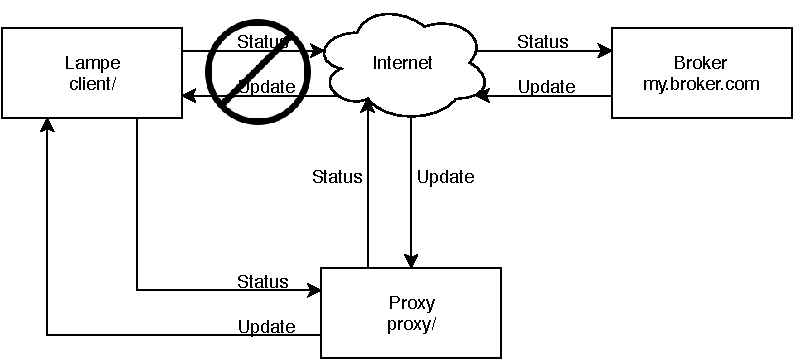
\includegraphics[width=14cm]{tex/bilder/2_grundlagen/Szenario1_MitM.pdf}
            \captionof{figure}{Darstellung eines Szenarios mit MITM}
            \label{fig:szenario-mitm}
        \end{figure}
        
    \subsection{Security Assessment}
        Um den Arbeitsablauf eines Penetration Tester aufzuzeigen, werden die 7 Schritte des \ac{PTES} \cite{hsiangchih_2019} beschrieben.
    
    \subsubsection{\glqq Pre-engagement Interactions\grqq{}}
        Es werden alle Vorbereitungen und Absprachen zum Umfang, wie Zeit und IP Adressen, und Art des Tests, Netzwerk- Web Penetration-Test, besprochen.
    \subsubsection{\glqq Intelligence Gathering\grqq{}}
        Hier werden so viele Informationen über das Ziel herausgefunden wie nur möglich. Dies ist notwendig um ein bestmögliches Bild über das Ziel zu bekommen und sich somit viele Angriffsvektoren einfallen lassen kann. Des Weiteren ist es auch essentiell, um nicht direkt aufzufallen da Sicherheitsmaßnahmen im Vorhinein identifiziert und möglicherweise umgangen werden können. Das reduziert die Aktionen, welche in Logdateien gespeichert werden und macht die Anwesenheit nicht so leicht identifizierbar. Als Beispiel ist es möglich eine Aktion mit zufällig generierten Werten aufzurufen. Dies würde allerdings eine Menge an fehlerhafter Anfragen dokumentieren, die offensichtlich nicht durch die Software auf Seite des Herstellers hervorgerufen wurde. Als Alternative ist es möglich die bestehende Kommunikation zu untersuchen und auf Basis der observierten Kommunikation vom Endgerät, leicht abgewandelte Versionen zu erzeugen. Hierbei hilft die konzipierte Software, als Alternative zu bestehenden Lösungen wie Wireshark um diese Kommunikation zu überwachen und Informationen über die Kommunikation zu erfassen.
    \subsubsection{\glqq Threat Modeling\grqq{}}
        Nachdem Informationen über den Dienst gesammelt wurden, ist der Tester nun in der Lage ein Modell zu entwickeln, indem mögliche Vertrauensstellung nicht ausreichend geschützt oder Input und Output nicht korrekt auf Sonderzeichen oder auch nicht auf Plausibilität geprüft werden könnte. 
    \subsubsection{\glqq Vulnerability Analysis\grqq{}}
        In diesem Schritt wird die Applikation auf Schwachstellen untersucht. 
        Dieser Schritt ist in zwei Teile, der Identifikation und der Prüfung, geteilt.
        Die Identifikation wird mithilfe von aktiven und passiven Methoden durchgeführt.
        Auf der einen Seite stehen Tools für aktive Tests wie zum Beispiel 
        SQLMap \cite{damele_stampar_2014}, 
        Burp Suite \cite{LozanoCarlosA.author2019Hapt}, %https://proquestcombo.safaribooksonline.com/book/web-development/9781788994064
        Nessus \cite{BealeJay2008Nna}, %https://proquestcombo.safaribooksonline.com/9781597492089
        \ac{ZAP} \cite{bennetts2013owasp}. %https://www.owasp.org/images/9/96/OWASP_2014_OWASP_ROMANIA.pdf
        Nachdem die Tools eingestellt sind, scannen und interagieren mit den Funktionalitäten der Seite oder Applikation ohne weitere Aktionen vom Nutzer.
        Auf der anderen Seite stehen die passiven Tools wie Wireshark oder TCPdump \cite{tcpdump_2010}, welche außenstehend sind und nur am Aufzeichnen von Aktionen anderer sind. 
        Diesen gemeldeten/ gefundenen Schwachstellen werden anschließend verifiziert, also auf die Korrektheit geprüft und zum Schluss anhand der Risiken aus aus Sicht der Applikation bewertet \cite{hayes_2012}.
    \subsubsection{\glqq Exploitation\grqq{}}
        In diesem Schritt wird versucht, unter Umgehen weitere Sicherheitsmechanismen, die bestätigte Schwachstelle so zu verwenden, dass entweder eine Steigerung der Berechtigungen oder das weiter Infiltrieren erreicht wird.
    \subsubsection{\glqq Post Exploitation\grqq{}}
        Im vorletzten Schritt wird versucht den erlangten Zugriff zu festigen und eventuelle benötigte Daten herunterzuladen. Das heißt, dass selbst nach dem Neustart des Systems die Kontrolle über das System bestehen bleibt ohne erneut den Exploit zu verwenden. Üblicherweise wird dies mithilfe von Tools wie einer \ac{RAT} gemacht, welche in den Autostart, die Registry geschrieben oder mithilfe von/ in Windows Komponenten integriert werden.
        Diese Programme ermöglichen die Steuerung des Computers ohne anwesend (vor dem Gerät) zu sein. Des Weiteren sind die Programme, sehr gut versteckt um nicht aufzufallen. Die Namen ähneln meist Dienst- oder Programmbezeichnungen um legitim auszusehen. Es gibt ebenfalls die Möglichkeit, das Programm so zu schützen, dass beim Versuch das Programm zu beenden das System selbst herunterfährt.
    \subsubsection{\glqq Reporting\grqq{}}
        Dies ist der letzte und einer der wichtigsten Schritte. Da Security Tests durchgeführt werden um die Sicherheit zu erhöhen, ist es auch zwingend notwendig die Schwachstellen und Exploits so zu dokumentieren, dass der Hersteller sich entscheiden kann, ob die existierenden Probleme behoben werden oder das Risiko getragen wird. Abhängig von dem Einfluss auf das Geschäft (auch Business Impact gennant) kann es aus wirtschaftlicher Sicht gerechtfertigt sein eine Schwachstelle nicht zu schließen und die daraus resultierenden Folgen wie Strafen zu bezahlen.

\section{IoT Security}
    \subsection{OWASP IoT Guide}
        Die OWASP Foundation \cite{guzman_2019} beschreibt das \ac{OWASP} wie folgt.
        \glqq OWASP is an open community dedicated to enabling organizations to conceive, develop, acquire, operate, and maintain applications that can be trusted. All of the OWASP tools, documents, forums, and chapters are free and open to anyone interested in improving application security. We advocate approaching application security as a people, process, and technology problem because the most effective approaches to application security include improvements in all of these areas.\grqq{}
        
        Das bedeutet, dass das Projekt eine offene Gemeinschaft ist, welche freie und unentgeltliche nutzbare Software zum Testen von IT Sicherheit bereitstellt. Darüber hinaus veröffentlichen sie ebenfalls jährliche Ranglisten bezüglich der am häufigsten vorgefundenen Schwachstellen des vergangenen Jahres. Ebenfalls werden Entwickler durch Informationen, oft auftretender Schwachstellen und dessen Behebung sowie Methodiken, unterstützt die für eine sichere Entwicklung und auch Architektur entscheidend sind. Die Ziele sind vor allem Personen auf die Probleme hinzuweisen, und sie somit zum kritischeren Nachdenken bringen sowie darauf Hinweisen vorsichtiger im Umgang mit digitalen Medien zu sein.
        
        Aus diesem Zusammenschluss vieler Sicherheitsexperten ist ebenfalls das Manufacturer \ac{IoT} Security Guidance Dokument \cite{stahl_2017} entstanden. Es beschreibt wie Hersteller von intelligenten Geräten sichere Produkte erstellen können. Es wird den Entwicklern ein Reihe an grundlegenden Richtlinien bereitgestellt, welche mindestens berücksichtigt werden sollten, um die Sicherheit stark zu erhöhen.
        Diese Inhalte zeigen, wieso \ac{IoT} Geräte im Jahr 2018 verwundbar sind und auf welche Angriffsvektor\footnote{Der Angriffsvektor ist die Methode, mit der ein Angriff sein Ziel erreicht \cite{HANSMAN200531}.} bei der Entwicklung berücksichtigt werden sollten. 
        Folgende Kategorien sind in 2018 nach \ac{OWASP} die Schwachstellen, welche am häufigsten vorkommen. 
        \begin{itemize}
            \item I1: Unsichere Weboberflächen
            
            Viele der Oberflächen, welche zum Konfigurieren der Geräte verwendet werden, beinhalten verschiedene Schwachstellen.
            Es sollten unsichere Passwörter verboten werden, ein Schutz gegen erraten von Passwörtern implementiert, und gegen bekannte weitere Schwachstellen geschützt und getestet werden.
            
            \item I2: Unzureichende Authentifizierung
            
            Grundlegend sollte es möglich sein, das vom Hersteller eingestellte Passwort durch einen Nutzer abzuändern.
            
            Des Weiteren werden Grundregeln für Passwörter bei der Auslieferung und Änderung empfohlen. Dies soll sicherstellen, dass nicht nur zur Inbetriebnahme sondern auch während der Verwendung des Produktes beim Endkunden der Zugriff zu privilegierten Funktionen und Bereichen unberechtigten effektiv verwehrt wird. Das Bundesamt für Informationssicherheit \cite{bundesamt_fuer_sicherheit_in_der_informationstechnik_2018} 
            empfiehlt als Minimum die folgenden Regeln.
            \begin{enumerate}
                \item Mindestens 8 Zeichen
                \item Großbuchstaben
                \item Kleinbuchstaben
                \item Zahlen
                \item Sonderzeichen (,.?!=()-...)
                \item Keine Wörter die im Wörterbuch stehen
            \end{enumerate}
            
            Des Weiteren wird eine zwei Faktor Authentifizierung als notwendig angesehen, für den Fall, dass das Passwort doch ausgelesen oder abgefangen wurde. Zwei Faktor bedeutet, dass ein zweiter Weg für die Bestätigung der Identität genutzt wird wie zum Beispiel eine SMS oder Benachrichtigung in einer Applikation über das Handy.
            
            \item I3: Unsichere Netzwerkdienste
            
            Dienste die ungeschützt im Netzwerk sind, sollten nur über die notwendigen Schnittstellen ansprechbar sein.
            Auch die dahinter liegenden Funktionen sollten auf die korrekte Prozessablauf und etwaige Fehlverhalten, zum Beispiel eine fehlerhafte Speicherbelegung, geprüft werden.
            
            \item I4: Fehlende Transportverschlüsselung
            
            Der Datenverkehr zwischen den Komponenten sowie den Geräten und dem Ziel sollte verschlüsselt sein um das Mitlesen oder Manipulieren der Nachrichten zu verhindern.
            
            Eine Verschlüsselungen zu verwenden hilft jedoch nicht immer beim erreichen der Sicherheitsziele Integrität, Vertraulichkeit. Nur für den Fall, dass die Verschlüsselung auch noch auf dem aktuelle Stand und noch nicht ausgehebelt wurde \cite{bsi_2019}.
            
            Für die sichere Übertragung steht SSL/TLS zur Verfügung welches verwendet werden sollte um ebenfalls eine Manipulation zu vermeiden. Dies ist in Bezug auf das \ac{MQTT} Protokoll ebenfalls möglich, jedoch nicht im Standard enthalten (siehe Kapitel 2.2.3).
            
            \item I5: Datenschutzbedenken
            
            Es soll sichergestellt werden, dass nur die nötigsten personenbezogenen Daten gesammelt und übertragen werden. Diese sollten dann auch anonymisiert werden um keinen Rückschluss auf die Person oder den Account schließend zu können.
            Selbstverständlich dürfen auch nur speziell zugelassene Personen die Daten erheben und übertragen können.
            Des Weiteren spielt auch im Bereich des Datenschutzes spielt die Verschlüsselung eine Rolle, denn die sensiblen Daten sollten zu jeder Zeit verschlüsselt sein.
    
            \item I6: Unsichere Cloud Schnittstellen \& I7: Unsichere Mobile Schnittstellen
            
            Weiterhin sollten die bereits erwähnten Richtlinien und Sicherheitsmechanismen (siehe \emph{I1: Unsichere Weboberflächen}) ebenfalls für die Kommunikationspartner oder entfernte Schnittstellen,  
            umgesetzt werden. Hinzukommt jedoch das die Übertragung zu diesem entfernten Gerät ebenfalls durch passende Sicherheitsmechanismen, wie TLS1.2 / TLS1.3, geschützt werden sollten.
            
            \item I8: Unzureichende Anpassungen im Bereich der Sicherheit
            
            Unzureichendes Loggen von Sicherheitsevents wie Angriffen oder Meldung über manipulierte oder unrealistische Nachrichten sind ebenfalls notwendig um rechtzeitig reagieren zu können. Der Nutzer sollte darüber schnellstmöglich informiert werden um entsprechende Maßnahmen einleiten zu können wie Passwörter ändern oder das Gerät vom Netz nehmen.
            
            Mithilfe dieser Maßnahmen wäre es ebenfalls möglich unberechtigte Aktivitäten Dritter schnellstmöglich zu unterbinden.
            
            \item I9: Unsichere Software/Firmware
            
            Es sollte ein Update-Mechanismus vorhanden sein, um bei bekannt werden von Schwachstellen das System oder die Applikationen mit einem nicht verwundbaren Programm auszutauschen. 
            Die installierte und übertragene Software oder Firmware sollte verschlüsselt und gesichert übertragen werden um eine Veränderung dieser zu verhindern.
            
            \item I10: Unzureichende Physische Sicherheit
            
            Selbstverständlich sind alle bereits genannten Methodiken zum Schützen des Gerätes unzureichend, für den Fall, dass Angreifer an das Gerät direkt kommen und somit die Software oder Hardware ändern können. Dies sieht man oft bei Wireless Access Points\footnote{\glqq Ein Wireless Access Points (WAP), auch WLAN Access Point oder kurz Access Point (AP) genannt, ist eine Funk-Basisstation innerhalb eines lokalen Netzwerks (LAN), um Clients über WLAN an das drahtgebundene Netzwerk anzuschließen.\grqq{} \cite{elektronik_kompendium_2018}}, welche ungesichert an der Wand oder auf dem Boden liegen.
        \end{itemize}
        
        Aus diesen ausgewählten Punkten ergeben sich eine Auswahl an entsprechenden Angriffsvektoren auf \ac{IoT} Geräte. Auf der anderen Seite gibt es ebenfalls Informationen für Sicherheitsprüfer oder -tester auf der Seite des \ac{OWASP} unter dem Namen \glqq IoT Testing Guides\grqq{} \cite{smith_2016}. Dieses Dokument gilt als strukturierter Leitfaden für die Suche nach Schwachstellen.
        
        \subsection{Internet of things (IoT) security}
        In dem Forschungsartikel \glqq IoT Security: Ongoing Challenges and Research Opportunities\grqq{} von Z. Zhang et al. \cite{6978614} beschreiben die Autoren das durch den Anstieg in dem Feld nicht nur die Angriffsfläche steigen wird sondern auch neue Angriffsvektoren hinzukommen.
        Sie nennen zwei Sicherheitsprobleme, welche eine entscheidende Rolle in Zukunft spielen werden.
        \begin{enumerate}
            \item Die Geräte
            
            Die Geräte verwenden eine Software, wo die Architektur nicht immer vollständig durchdacht oder mit Fokus auf Sicherheit entwickelt wurde. Dies kann zu Schwachstellen und dadurch Kompromittierungen von Daten der Geräten führen. Bereits gelöste Probleme kommen wieder zum Vorschein, da die Geräte nicht die gleichen Spezifikationen haben wie die, die wir jeden Tag verwenden um uns die Arbeit zu erleichtern. 
        
            Es ist laut einer Umfrage von Statista \cite{kaspersky_lab_2019}
            heutzutage oft der Fall, dass Antivirus Software zum Schutz des Computers oder Smartphone verwendet werden. Diese Software benötigt allerdings viele Ressourcen um verwendet werden zu können.
            Kaspersky \cite{ao_kaspersky_lab_2018_1}
            als Beispiel, setzt 1150 MB Festplattenspeicher mit einem Intel/AMD 32/64 Bit Prozessor mit 1 GHz und 1 GB freien Arbeitsspeicher nur für die Funktionalität der Software voraus. Es ist davon auszugehen, dass bei Geräten die für einen speziellen Einsatzzweck optimiert sind, keine Hardware verbaut wird die mehr als das nötigste leisten kann um das Produkt entsprechend preiswert anbieten zu können. Dies ist notwendig, da zum Beispiel der Markt im Bereich Sprachsteuerungen laut Futuresource Consulting \cite{futuresource_consulting_ltd_2019}, mit fünf Geräten von drei verschiedenen Herstellern, hart umkämpft ist. Schaut man sich den Stromverbrauch des Amazon Echo Dot \cite{amazon_de_alle_produkte_2018} an, fällt auch recht schnell auf, dass 15 W nicht mit einem Computer mithalten kann. 
            Der Microcontroller Raspberry Pi 2B \cite{raspberry_pi_foundation_2016}, welcher auch gerne dazu verwendet um \ac{MQTT} Projekte umzusetzen, lässt auch eine Diskrepanz in der technischen Spezifikationen in mehreren Punkten erkennen. Der Prozessor besitzt eine ARM Architektur, taktet mit 900 MHz 
            und ist 32 Bit fähig. Der Prozessor entspricht also den Mindestanforderungen der Architektur nicht und würde weiterhin der eigentlichen Anwendung auf dem Gerät eine zu geringe Performance ermöglichen. Des Weiteren entspricht auch der Arbeitsspeicher von 1 GB nicht den Mindestanforderungen.
            Somit kommen Sicherheitsprobleme, welche in der Vergangenheit bereits gelöst wurden, erneut zum Vorschein und bedürfen einer neuen Lösung.
            
            Zusätzlich zu den Sicherheitsmechanismen, welche nun nicht mehr verwendet werden können, sind \ac{IoT} Geräte nicht nur von einem Typ. Es gibt viele verschiedene Hersteller und Geräte die sich in den Funktionen, Erscheinungen und Spezifikationen unterscheiden. Diese heterogene Landschaft erhöht die Komplexität, eine Lösungen für alle Geräte zu finden oder den Aufwand für jedes Gerät einen eigenen Sicherheitsmechanismus zu implementieren.
            
            \item Die Kommunikation
            Die heterogene Landschaft beeinflusst jedoch nicht nur die Komplexität auf der Seite der Geräte sondern auch in Bezug auf die Kommunikation.
        
            Es ist denkbar, dass der Wecker mit den Rollläden kommunizieren kann, dieser wiederum die Fenster dazu bringt sich zum Lüften zu öffnen. Automatisch wird die Kaffeemaschine und das Radio angeschaltet damit der Besitzer Kaffee während den neuesten Meldungen genießen kann.
            Nur dieser einzelne Prozess beinhaltet bereits fünf verschiedene Geräte, welche im ersten Moment nichts miteinander zu tun haben. Doch sind alle voneinander abhängig und der Prozess kann durch das manipulieren eines einzelnen Gerätes in der Kette, entweder gestoppt werden oder auch zu einem ungewollten Ergebnis führen.
            
            Ein Problem innerhalb der Kommunikation ist die Identifikation der Geräte. Aktuell wird \ac{DNS} zum Auflösen der Hostnamen auf die dazugehörige IP-Adresse verwendet. Dieses System ist allerdings anfällig gegen Attacken wie DNS cache poisoning oder \ac{MITM} und somit auch nicht sicher.
            DNS cache poisoning bedeutet, dass durch manipulierte DNS Antworten der Zwischenspeicher, welcher die Gegenüberstellung von IP und Hostnamen besitzt verändert wird. Die Folge daraus ist, dass nicht mehr die IP Adresse des legitime Ziels neben dem Namen (z.B. google.de) sondern die IP Adresse des Angreifers steht und somit auf den Angreifer weiterleitet.
            \ac{DNSSEC} wird von der zentralen Registrierungsstelle für die deutsche Domainendung \glqq .de\grqq{} \cite{denic_eg}
            als \ac{DNS} Zusatz beschrieben, der verwendet wird um sicherzustellen, dass der Eintrag sowie der Transportweg zwischen der legitimen Adresse und dem DNS-Server geschützt ist und sich kein dritter Akteur einmischen kann.
        
    \end{enumerate}
    %Zusätzliche Quellen%
    %A Survey on the Internet of Things Security: https://ieeexplore.ieee.org/abstract/document/6746513
    %Blockchain for IoT security and privacy: The case study of a smart home: https://ieeexplore.ieee.org/abstract/document/7917634
    %A Critical Analysis on the Security Concerns of Internet of Things (IoT): http://www.pcporoje.com/filedata/592496.pdf
    %Internet of things (IoT) security: Current status, challenges and prospective measures: https://ieeexplore.ieee.org/abstract/document/7412116
    %A Systemic Approach for IoT Security: https://ieeexplore.ieee.org/abstract/document/6569455
    %Security analysis on consumer and industrial IoT devices: https://ieeexplore.ieee.org/abstract/document/7428064
    %Botnets and Internet of Things Security: https://www.computer.org/csdl/magazine/co/2017/02/mco2017020076/13rRUxZRbvu

\section{Bestehende Lösungen}
    %Implementierungen auf dem Markt
    Im Folgenden wird auf zwei Implementierungen eingegangen die das Ziel haben, Nachrichten des \ac{MQTT}-Protokolls an ein drittes Gerät weiterzuleiten.
    Diese ist interessant, da diese Funktionalität im Standard \cite{gupta_banks_2015} nicht unterstützt wird. Durch das publish/subscribe Prinzip ist der Broker nicht in der Lage, selbst kommunizieren zu können. Er kommuniziert ausschließlich die neuen Nachrichten an die abonnierten Geräte weiter und kann nicht selbst Nachrichten schicken.
    
    \subsection{MQTT Bridges}
        Dadurch haben mehrere MQTT Bibliotheken \cite{84codes_ab_2016} \cite{light_2019} erkannt, dass die Funktionalität für das Weiterleiten von Nachrichten an einen weiteres Gerät sehr hilfreich ist. Als Beispiel wird diese Funktionalität benötigt, um Geräte, welche \ac{MQTT} als Protokoll haben, mit anderen Geräten sprechen zu lassen und somit von dem Status des einen Geräts abhängige Abläufe zu ermöglichen.
        Um dieses Problem zu lösen, haben die Bibliotheken das MQTT Bridge Feature hinzugefügt. Es besteht aus einem Client der an den Broker angeschlossen wird. Mithilfe von modifizierten Events, die aktiviert werden sobald der Broker eine Nachricht empfängt, können die Nachrichten direkt an einen zusätzlichen Client weitergeleitet werden der die sich mit dem dritten Broker verbunden hat.
    
    \subsection{Axway - API Management Plus}
        Die API-Management Software von Axway vereint das Erstellen und Organisieren vieler verschiedener Schnittstellen mit direkten Anbindungsmöglichkeiten für Endgeräte. Darüber hinaus, können alle Endpunkte auf fehlerhaftes Verhalten oder Anfragen geprüft werden. Dies soll es möglich machen, auf die schnellen Änderungen auf dem Markt eingehen und viele verschiedene Geräte parallel unterstützen zu können.
        Um auch intelligente Geräte aus dem \ac{IoT}-Bereich unterstützen zu können, wurde ein Proxy für das Protokoll \ac{MQTT} entwickelt \cite{axway_2018} Der Proxy befindet sich zwischen dem Client und dem Broker. Dadurch hat er die Möglichkeit die eingehenden Pakete abzufangen und anhand eines Regelwerks, welches per REST über den API Manager erreichbar ist, Daten zu validieren.
        
        Das Ziel dieser Lösung ist somit, auf Basis der Richtlinien welche auf dem Management-Server hinterlegt werden, gesendeten Nachrichten des \ac{MQTT} Protokolls zu filtern und nicht regel konforme Kommunikation zu blocken. Dies könnte bedeuten, dass nur spezielle Geräte ein Thema abonnieren können und somit dem Protokoll die Möglichkeit geben, Rechte und Berechtigungen zu verteilen.
        
        Die Lösung wird in verschiedenen Versionen als Docker-Container bereitgestellt. Für den Fall, dass bereits ein eigener Broker und ein Regelwerk im Einsatz ist, kann der \ac{MQTT}-Proxy als alleinstehend betrieben werden. Fall jedoch alle Systeme benötigt werden, können Broker, Regelwerk und Proxy auf einmal aufgesetzt werden, um eine direkte Testumgebung bereitzustellen.
        
        Jedoch besitzt diese Lösung gewisse Einschränkungen.
        Es ist zum Beispiel nicht möglich:
        \begin{itemize}
            \item Mehrere Broker per Proxy Instanz zu definieren
            \item TLS support zwischen Client und Proxy sowie Proxy und Broker zu ermöglichen
        \end{itemize}
        
        Trotz den Einschränkungen ist es möglich bei einer unverschlüsselten Kommunikation Daten abzufangen, deren Inhalt auswerten zu können und anhand von Regeln Pakete zu verwerfen.
        
        Der Datenflow sieht wie folgt aus.
        \begin{figure}[h]%h=direkt danach t=top b=bottom
            \centering
            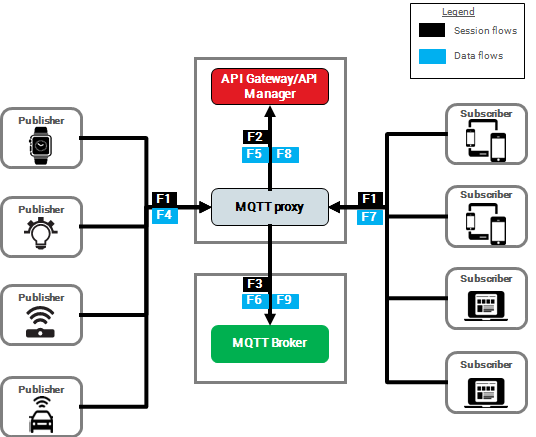
\includegraphics[width=14cm]{tex/bilder/2_grundlagen/axway-mqtt-proxy02_short.png}
            \captionof{figure}{Datenflow des Axway MQTT Proxies \cite{axway_2018}}
            \label{fig:axway-proxy}
        \end{figure}
        \begin{itemize}
            \item F1: Das \ac{IoT}-Gerät (oder auch Client genannt) sendet eine Connect-Nachricht mit Benutzerdaten zum Proxy um sich damit zu verbinden
            \item F2: Die Benutzerdaten werden zum verifizieren dem API Gateway gesendet
            \item F3: Mit der Bestätigung vom Gateway wird die Session zum Proxy hergestellt.
            \item F4: Das Gerät sendet eine Nachricht an den Proxy.
            \item F5: Der Proxy verifiziert bzw. ändert die Nachricht auf Basis der Gateway Regeln.
            \item F6: Die Nachricht wird an den externen Broker weitergeleitet.
            \item F7: Um nun eine Antwort zu erhalten sendet der Client eine Subscribe Nachricht an den Proxy
            \item F8: Der Proxy verifiziert bzw. ändert die Nachricht auf Basis der Gateway Regeln.
            \item F9: Der Proxy leitet die Nachricht an den externen Broker weiter.
        \end{itemize}
    %Analyse der Lösung
    %Dieses Implementierung besitzt bereits die Möglichkeit, Daten abzufangen und den Inhalt auswerten zu können, so wie es ebenfalls in dieser Arbeit vorgesehen ist. Die gleichen Einschränkungen, welche die Lösung von Axway hat, wird auch in dieser Arbeit als Voraussetzung definiert: Es ist nicht ohne weiteres möglich ist, die Zertifikate, welche für eine TLS geschützte Verbindung mit dem Broker benötigt werden, zu erhalten. Da bei \ac{IoT} Geräten der Hersteller die Kontrolle über den Server und somit über die Zertifikate hat.
    %Was darüber hinaus jedoch nicht von API Management Plus angeboten wird, sind die folgenden Funktionen, welche im Rahmen eines Security Audits benötigt werden: 
    %\begin{itemize}
        %\item HTTP Schnittstelle zum senden selbst erzeugter Nachrichten an das gewählte Ziel.
        %\item Erneute versenden von bereits gesendeten Nachrichten um Nebeneffekte oder zustandsabhängige Funktionen zu erkennen.
        %\item Manuelle Manipulation der ausgehenden und ankommende Pakete.
    %\end{itemize} % Externe Datei einbinden
\chapter{Anforderungserhebung}

\section{Nutzer}
%Thesis Fragestellung aufgegriffen
    Um die Frage beantworten zu können, ob es möglich ist die übertragenen Daten der intelligenten Geräte, herstellerübergreifend überwachen zu können, ist es nötig Zugriff auf die eingehenden, sowie ausgehenden Daten der Geräte zu erhalten. In diesen Daten, welche vom \ac{IoT}-Gerät zum Broker und anders herum, geschickt werden befinden sich möglicherweise personenbezogene Daten sowie Hinweise auf mögliche Schwachstellen.
    Die nächste Herausforderung ist die gesammelten Daten auch einem Nutzer in einer aufbereiteten Ansicht zugänglich zu machen und die direkte Interaktion mit den Daten zu ermöglichen.

    Aus diesem Szenario heraus ergeben sich zwei wichtige Nutzerrollen.
    
%=====================================================================%    
%Wer? Nutzerrolle: Admin (monitoring)
%=====================================================================%    
    Auf der einen Seite existiert der System- , Netwerkadministrator, welcher versucht Probleme in der Kommunikation zu finden und zu lösen oder eventuelle Anomalien zu erkennen.
%Aufgabenbereiche Motivation
    Nach Burgess \cite{burgess2004principles} zählen zu den Aufgabenbereichen von Netzwerk- und Systemadministratoren zählen unter anderem:
    \begin{itemize}
        \item \glqq Diagnostics, fault and change management\grqq{}
        
        Die Aufgabe der Administratoren in einem Unternehmen besteht unter anderem darin, Systeme für das eigene Unternehmen oder Kunden bereitzustellen und bei Problemen zu helfen. Um bei Problemen herausfinden zu können, wo das Problem entstanden ist und wie es schnell behoben werden kann, ist es hilfreich die Kommunikation im Netzwerk zu beobachten. Zum Beispiel kann erkannt werden, ob \ac{TCP}-Pakete überhaupt an dem Gerät ankommen oder schon auf dem Übertragungsweg verloren gehen. Abhängig davon, kann das Problem weiter eingeschränkt und irgendwann lokalisiert werden.
        
        \item \glqq Configuration and maintenance\grqq{}
        Für eine korrekte Konfiguration der Systeme ist es notwendig die Kommunikation nachvollziehen zu können. Dazu muss ein Verständnis der genutzten Technologien vorhanden sein. Des Weiteren sollte ebenfalls bekannt sein, welche Art von Daten mithilfe der Kommunikation übertragen werden.
        
        %Performance regarding bottlenect.
        Die Aufzeichnung von Datenpaketen, deren Größe und Zeitstempel ermöglichen mithilfe von statistischer Analyse, Rückschlüsse auf die Netzwerkbelastung.
        
        \item \glqq Application-level services\grqq{}
        
        %Reverse Proxies und DNS
        Auf dieser Ebene müssen Administratoren verschiedene Applikationen wie \ac{DNS}-Server\footnote{\glqq Das DNS verknüpft [...] Rechnernamen und IP-Adressen miteinander. Es leistet zusätzlich die Speicherung und Ausgabe weiterer Informationen über die Dienste, die mit einer Domain verknüpft sind.\grqq{} \cite{denic_eg}} oder Proxies konfigurieren und Anwendungen miteinander verbinden um neue Systeme in die bestehende Systemlandschaften zu integrieren.
        
        \item \glqq Network-level services\grqq{}
        
        Auch können verschiedene Protokolle miteinander verbunden werden.
        
    \end{itemize}

% Ziel
    Das Ziel eines Netzwerkadministrators ist somit die Identifikation von Störquellen sowie das sicherstellen der Verfügbarkeit aller geschäftskritischen Dienste (\emph{high availability}). Dies ist eine wichtige Voraussetzung für hohe Kundenzufriedenheit.
    
%was gibt es bereits (Wireshark) was kann die Software besser/kann nur die Software
    Wie bereits erwähnt, gibt es für die einzelnen Phasen verschiedene Tools die sich in der Praxis bereits etabliert haben und Anwender in ihrer Arbeit unterstützen.
    
    %https://proquestcombo.safaribooksonline.com/9781492020356
    Wireshark \cite{SandersChris2017Ppa}, ein Tool zum Überwachen und Aufzeichnen des Netzwerkverkehrs, beinhaltet die gleiche Funktionalität wie ein Teil der Proxy Komponente. Der unterschied besteht jedoch darin, das die Komponente zusätzlich direkt in die Kommunikation eingreifen können soll. Das bedeutet, dass Nachrichten verändert, fallengelassen oder erneut gesendet werden soll, was durch ein dediziertes Monitoring-Tool nicht möglich ist.
    
% Was müsste die eigene Software verbessern
    %Log Messages
    Der Nutzer möchte nun, wenn er mit diesem Programm arbeitet, den Proxy in den Modus \glqq intercept\grqq{} oder \glqq none intercept\grqq{} stellen können um Inhalte spezieller Clients einzeln und gezielt prüfen zu können ohne zu viele Daten anderer Geräte im Netzwerk zu erhalten.
    %View Messages
    Des Weiteren möchte der Nutzer die Nachrichten, welche durch den \glqq intercept\grqq{} Modus abgefangen wurden, aufgelistet und angezeigt werden.
    %View ClientInfos
    Für denn Fall, dass etwas nicht ordnungsgemäß funktioniert oder fehlerhaft Konfiguriert wurde, ist es ebenfalls relevant die Verbindungsdaten der einzelnen Proxy Clients mit einer Verknüpfung mit dem zu untersuchenden \ac{IoT}-Gerät einsehen zu können.
    
%=====================================================================%
%wer? Nutzerrolle: Security Auditor
%=====================================================================%
% Motivation
    Auf der anderen Seite existiert der Security Auditor oder auch Penetration Tester, welcher versucht Schwachstellen in der Kommunikation oder dem Gerät oder dem Endpunkt zu identifizieren.
% Ziel
    Dies ermöglicht auf der einen Seite den Hersteller, von dem der Tester beauftragt wird, die Produkte im Rahmen der Qualitätssicherung vor Veröffentlichung zu testen um Probleme zu vermeiden. Dies ist nicht für Vertrauen innerhalb der Branche wichtig, sondern auch in bestimmten Bereichen z.B. kritischen Infrastrukturen im Gesetz verankert.
    Auf der anderen Seite bestätigt es ebenfalls, dass der Dienst eines Unternehmens gute und effiziente Sicherheitsmechanismen korrekt implementiert hat um die Kundendaten vor Gefährdungen der Vertraulichkeit, Integrität oder Verfügbarkeit zu schützen.
    
    Eine weiterer wichtiger Untersuchungsgegenstand sind Personen- und Unternehmensbezogene Daten. Diese haben aufgrund von datenschutzrechtlichen Bestimmungen eine besonders hohe Priorität. Dies wird in Form von manueller oder regelbasierter Inspektion der Übertragung durchgeführt.
    
%Was für Arbeitsabläufe
    
    %wie: Wie hilft die Software dabei das Ziel zu erreichen
    Die in dieser Arbeit zu konzipierende Software soll den Tester mithilfe von passivem Scannen und abfangen der Kommunikation in Schritt 2 (\emph{Information Gathering}) und durch manipulieren sowie erneut senden der Nachrichten Schritt 5 (\emph{Exploitation}) unterstützen.
    
    %was gibt es bereits (Wireshark) was kann die Software besser/kann nur die Software
    Wie beim Netzwerkadministrator bereits geschildert, kann Wireshark zur Informationsbeschaffung verwendet werden.
    Da bei Wireshark viele verschiedene Protokolle unterstützt und auch sehr detaillierte Informationen angezeigt werden, passiert es schnell, dass durch die große Menge wichtige Bestandteile untergehen (auch \emph{visual clutter} genannt) oder nur mit Aufwand gefunden werden.
    
    Burp Suite von PortSwigger bietet im Gegensatz zu Wireshark ebenfalls eine Proxy Komponente und kann somit, wie in diesem Tool geplant, die Nachrichten protokollieren bzw. überwachen sondern auch in die Kommunikation eingreifen. Der große Unterschied besteht darin, dass Burp Suite ausschließlich für HTTP/s und (Sec)Websocket Kommunikation zu verwenden ist und keinerlei Unterstützung für das \ac{MQTT}-Protokoll bietet. Man könnte die Idee jedoch am einfachsten mit dieser Lösung vergleichen, da auch eine ähnlich Bedienung von Vorteil wäre. Dadurch würden Nutzer eine geringere Einarbeitungszeit benötigen und auch die Akzeptanz steigern.

\section{Abgeleitete Anforderungen}
    Im Folgenden werden die werden Use-Cases aus den obigen Nutzerbeschreibungen extrahiert und beschrieben.
    %Aus Beschreibung ergeben sich Use-Cases
    \subsection{Use-Cases}
    \begin{figure}[h]%h=direkt danach t=top b=bottom
        \centering
        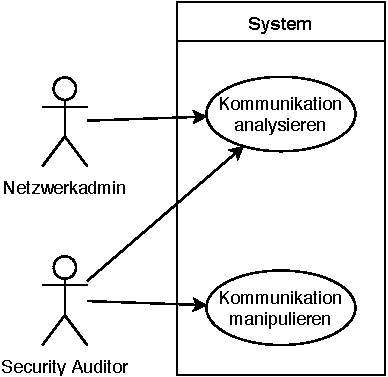
\includegraphics[width=7cm]{tex/bilder/3_anforderungen/Use-Case.pdf}
        \captionof{figure}{Use-Case Diagramm}
        \label{fig:use-case}
    \end{figure}
    
    Zum ersten Use-Case \emph{Kommunikation analysieren}:
    	Der Nutzer möchte die Nachrichten der \ac{MQTT}-Kommunikation analysieren.
    	Des Weiteren ist es notwendig das Abfangen der Nachrichten pro Gerät einstellen zu können, um nur die gewünschte Kommunikation und somit eine selektive Analyse zu ermöglichen.
    	Um dies zu bewerkstelligen, ist es notwendig die angezeigten Nachrichten nach den Inhalten zu filtern.
    	
    Zu \emph{Kommunikation manipulieren}:
        Im Folgenden werden Aktionen wie Payload ändern, Nachricht senden, Nachricht kopieren, Nachricht ändern bzw. speichern,Nachricht verwerfen beschrieben.
    	Der Nutzer möchte auf verschiedene Weisen die Kommunikation zwischen zwei Kommunikationspartnern über ein drittes System verändern können.
    	Durch Veränderung des Nachrichteninhalts einzelner Nachrichten ist es dem Nutzer möglich die Kommunikation zu verändern.
    	Anhand von selbsterstellten Pakete, welche im Namen der Kommunikationspartner erstellt werden, sollen vom Nutzer gewünschte Informationen übertragen werden.
    	Um die repetitive Arbeit der Nachrichtenerstellung zu reduzieren und die Arbeit zu beschleunigen, kann eine abgefangene Nachricht kopiert werden.
    	Diese Änderungen sollen anschließend gespeichert werden können um Nachrichten zu einem späteren Zeitpunkt versenden oder weiter Verändern zu können.
    	Für den Fall, dass übertragene Nachrichten Inhalte beinhalten, welche nicht ankommen dürfen oder nicht den gewünschten Inhalt haben, möchte der Nutzer sie verwerfen und somit von der Kommunikation entfernen.

    %Tabelle mit Funktionale Anforderungen
    \subsection{Formale Anforderungen} \label{FormaleAnforderungen}
    Anhand der Use-Cases lassen sich folgende formale Anforderungen ableiten (siehe Tabelle \ref{tab:functional_requirements}).
    Dabei ist zu beachten, dass diese Anforderungen, dadurch das es sich um ein abstraktes Konzept handelt, unspezifisch und ausschließlich funktional sind.
    \begin{table}[h]
        \centering
        \begin{tabular}{c|c}
            \hline
            $Nr.$ & $Name$ \\ \hline
            %Nachricht abfangen vllt auch ein Feature was nennenswert ist oder wird es m it Nr.3 abgedeckt???
            1 & Nachrichten anzeigen \\ \hline
            2 & Nachrichten filtern \\ \hline
            3 & Abfangen umschalten \\ \hline
            4 & Nachricht manipulieren \\ \hline
            5 & Nachricht senden \\ \hline
            6 & Nachricht verwerfen \\ \hline
        \end{tabular}
        \caption{Funktionale Anforderungen}
        \label{tab:functional_requirements}
    \end{table}
    
        \subsubsection{1. Nachrichten anzeigen}
        Das System ermöglicht die Anzeige von Nachrichten einer \ac{MQTT}-Kommunikation.
        Dabei werden diese in einer chronologischen Reihenfolge dargestellt und stellen relevante Informationen wie Topic, Payload, Quality of Service und Zeitpunkt der Übertragung zur Verfügung.
        In dieser Arbeit werden jedoch nicht alle eingehenden, sondern nur aktiv abgefangene, Nachrichten betrachtet, da diese die höchste Priorität besitzen.
        
        \subsubsection{2. Nachrichten filtern}
        Die Software muss angezeigte Nachrichten nach deren Attributen filtern können.
        
        \subsubsection{3. Abfangen umschalten}
        Dem Nutzer muss die Möglichkeit gegeben werden, das Abfangen der  Kommunikation der \ac{IoT}-Geräte zu aktivieren oder deaktivieren.
        Dabei werden die Pakete nicht nur dupliziert, sondern dürfen auch nicht an den Kommunikationspartner weiter geleitet werden.
        Dies muss dem Nutzer pro verbundenem Gerät zur Verfügung konfigurierbar sein.
        
        \subsubsection{4. Nachricht manipulieren}
        Der Nutzer muss den Inhalt der aufgezeichneten Nachrichten verändern können.
        Vorrangig muss der übertragene Nachrichteninhalt als Text verändert werden können.
        
        \subsubsection{5. Nachricht senden}
        Es muss garantiert werden, dass eigene Nachrichten gesendet werden können.
        Das Senden beinhaltet nicht nur das senden neuer Nachrichten, sondern umfasst auch das erneute senden (auch \emph{replay attack} genannt) von bereits übertragenen Nachrichten. Die Inhalte werden in diesem Fall nicht verändert und wie erfasst erneut versendet.
        
        \subsubsection{6. Nachricht verwerfen}
        Das System muss es dem Nutzer ermöglichen, abgefangene Nachrichten verwerfen zu können.
        Dies bedeutet, dass gesendete Inhalte nicht an den gewünschten Kommunikationspartner weitergeleitete werden, sondern nachdem sie abgefangen wurden aus der Kommunikation entfernt werden.
        Die ausgewählten Nachrichten werden somit auch in der Oberfläche nicht weiter angezeigt.
        
        
\chapter{Konzept}
In diesem Kapitel wird anhand der in Kapitel 3 erfassten Anforderungen ein Konzept entworfen. Nach der Beschreibung des Aufbaus wird der interne Ablauf, anhand von Diagrammen, detaillierter betrachtet.

\section{Aufbau der Software}
    Das in Abbildung \ref{fig:use-case} dargestellte Use-Case-Diagramm und die daraus abgeleiteten Anforderungen werden in diesem Kapitel zum Aufbau eines Konzepts verwendet.
    Hierbei wurde zunächst ein Systemdiagramm aus dem Use-Case-Diagramm abgeleitet (siehe Abbildung \ref{fig:system_all}).
    
    \begin{figure}[h]%h=direkt danach t=top b=bottom
        \centering
        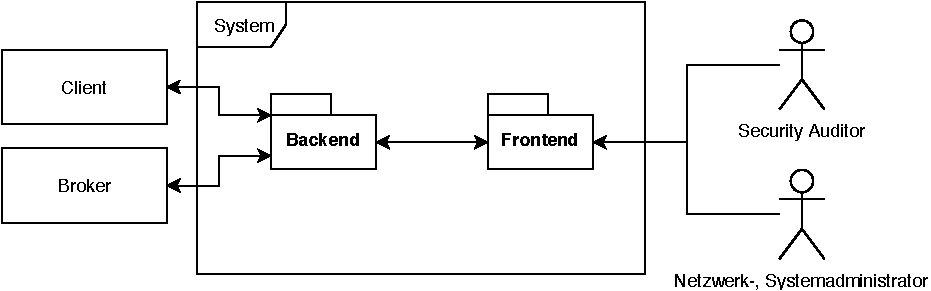
\includegraphics[width=14cm]{tex/bilder/4_konzept/Systemdiagram.pdf}
        \captionof{figure}{Systemdiagramm}
        \label{fig:system_all}
    \end{figure}
    
    Die Akteure (\emph{Netzwerk-, Systemadministrator} und \emph{Security-Auditor}) konnten direkt aus dem Use-Case-Diagramm übernommen werden.
    Sie stellen die mit dem System interagierenden Nutzer dar und kommunizieren direkt mit einem Frontend.
    Es erfolgt eine klare Trennung zwischen Backend und Frontend, damit Logik und Visualisierung voneinander unabhängig implementiert werden können.
    
    Das \emph{Backend} kommuniziert durch einen Proxy mit dem Client und empfängt die gesendeten Nachrichten. Anschließend verarbeitet es diese (führt die Manipulation der Daten durch) und leitet die verarbeiteten Nachrichten an den Broker des Betreibers weiter. Sobald eine Antwort zurückkommt, wird diese erneut bearbeitet und anschließend veröffentlicht.
    Die Hauptaufgaben des Backends sind die Datenhaltung (unter anderem Speicherung der Nachrichten, Verwalten der Clients) und die Verwaltung des Nachrichtenflusses zwischen allen beteiligten Kommunikationspartnern.
    
    Das \emph{Frontend} hingegen dient nur zur Visualisierung der Nachrichten und Clients sowie zur Interaktion mit dem Nutzer. Hierbei bezieht es die gespeicherten und neu eintreffenden Nachrichten vom Backend.

    \begin{figure}[h]%h=direkt danach t=top b=bottom
        \centering
        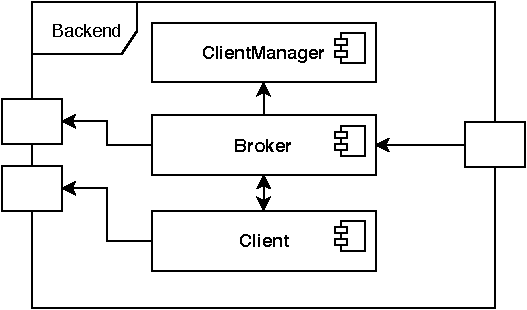
\includegraphics[width=8cm]{tex/bilder/4_konzept/Systemdiagramm_Konzept_Backend.pdf}
        \captionof{figure}{Komponentendiagramm Backend}
        \label{fig:system_backend}
    \end{figure}
    
    Abbildung \ref{fig:system_backend} zeigt eine Verfeinerung des Backends. 
    Durch das \emph{Publish/Subscribe}-Programmiermuster des \ac{MQTT}-Protokolls ist es notwendig, für jedes verbundene Gerät zwei Clients zu erzeugen, die die Nachrichten an den Betreiber übermitteln und die veröffentlichten Nachrichten wieder an den Broker des Proxys übermitteln.
    
    Einer der Clients (in diesem Fall \emph{ClientOut}) repräsentiert das tatsächliche Gerät und täuscht dies gegenüber der Endstelle des Betreiber vor. Dieser virtuelle Client übernimmt somit die Übertragung der Nachrichten zwischen dem Broker und dem Betreiber. Daraus resultiert, dass Nachrichten in gegengesetzter Richtung ebenfalls an den \emph{ClientOut} gesendet werden, auch an das physische Gerät weitergeleitet werden müssen. Dazu dient der zweite virtuelle Client (\emph{ClientIn}). Dieser erhält die vom \emph{ClientOut} erhaltene Nachricht an den Broker weiter mit der Folge, dass dieser die Nachricht anschließend veröffentlicht. Dabei muss sichergestellt werden, dass die vom Betreiber gesendete Nachricht nicht erneut nach außen gesendet wird.
    Eine grafische Darstellung des Prozesses ist Abbildung \ref{fig:aktivitaetsdiagramm_message} zu entnehmen.
    
    Der \emph{ClientManager} ermittelt die externen Clients zu den dazugehörigen \emph{ClientIn}- und \emph{ClientOut}-Instanzen. Damit wird sichergestellt, dass die Kommunikation mit dem externen Broker stattfinden kann.

    
    Abbildung \ref{fig:system_frontend} stellt die Komponenten des Frontends dar. Alle drei Komponenten sind voneinander unabhängig und arbeiten mit unabhängigen Informationen.
    
    Die \emph{Clients}-Komponente enthält die Informationen der virtuellen Clients (\emph{ClientIn} und \emph{ClientOut}). Diese werden, sobald der Nutzer die Seite besucht, vom Backend geladen und anschließend angezeigt. Sie ermöglicht ebenfalls die Konfiguration der abzufangenden Kommunikation pro Gerät.
    
    Die \emph{NewMessages}-Komponente ermöglicht das Erzeugen von neuen Nachrichten auf der Seite des Frontends und überträgt am Ende alle Informationen an das Backend, wo diese weiter verarbeitet (z.B. versendet) werden.
    
    Der \emph{Interceptor} ist für die Anzeige der abgefangen Nachrichten zuständig. Zu Beginn werden alle bestehenden Nachrichten abgefangen und, um das wiederholte Laden der Webseite zu verhindern und die Aktualität der Inhalte zu gewährleisten, dynamisch alle weiteren eingehenden Nachrichten nachgeladen. Um die Anzeige noch weiter strukturieren zu können, werden verschiedene Filter zur Verfügung gestellt, welche auf die Nachrichteninhalte und -attribute angewendet werden können.
    \begin{figure}[h]%h=direkt danach t=top b=bottom
        \centering
        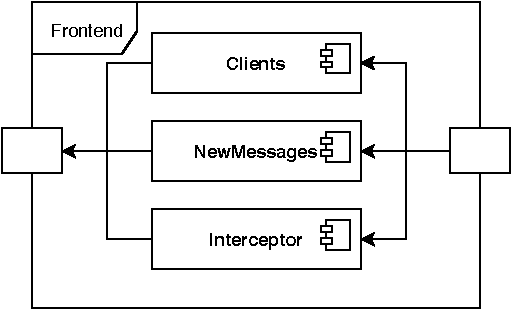
\includegraphics[width=8cm]{tex/bilder/4_konzept/Systemdiagramm_Konzept_Frontend.pdf}
        \captionof{figure}{Komponentendiagramm vom Frontend}
        \label{fig:system_frontend}
    \end{figure}

\section{Prozess}
    Im Folgenden wird der interne Ablauf des zu entwickelnden Systems (auch Proxy genannt), bestehend aus dem darin enthaltenen Broker, \emph{ClientIn} und \emph{ClientOut}, beschrieben.

    Das Aktivitätsdiagramm \ref{fig:aktivitaetsdiagramm_connect} veranschaulicht den Ablauf des Verbindungsprozesses nach der Verbindungsanfrage des Clients und terminiert mit dem erfolgreichen Verbindungsaufbau.
    Sobald ein \ac{IoT}-Gerät eine Verbindung zum Broker des Backends aufbaut, werden zwei virtuelle Clients (\emph{ClientOut} und \emph{ClientIn}) erzeugt.
    
    \begin{figure}[!h]%h=direkt danach t=top b=bottom
        \centering
        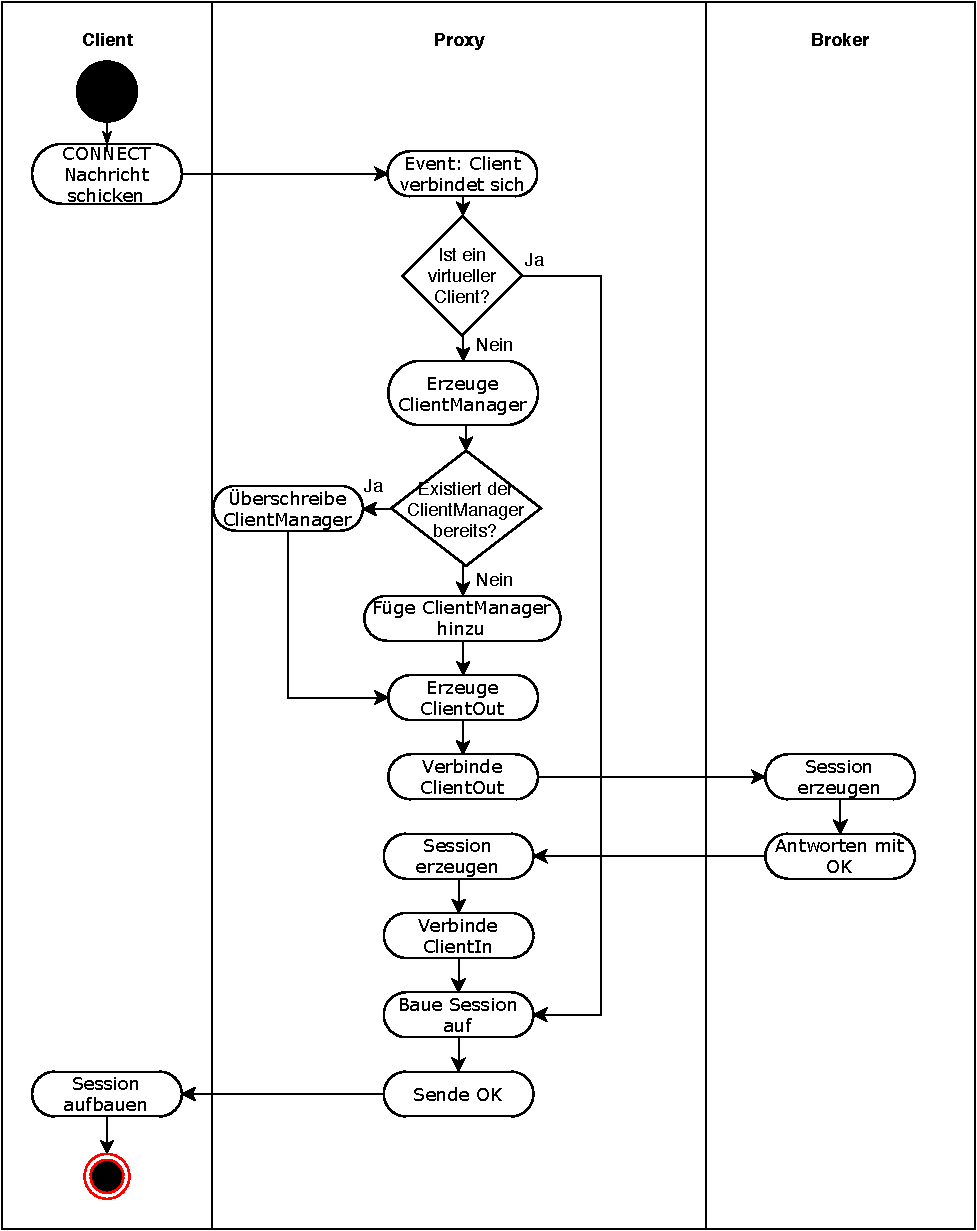
\includegraphics[width=14cm]{tex/bilder/4_konzept/Activity_Connect.pdf}
        \captionof{figure}{Aktivitätsdiagramm für das Event \glqq Client verbindet sich\grqq{}}
        \label{fig:aktivitaetsdiagramm_connect}
    \end{figure}
    %%%%%%%%%%%%%%%%%%%%%%%%
    \newpage
    %%%%%%%%%%%%%%%%%%%%%%%%
    Das nächste Diagramm (\ref{fig:aktivitaetsdiagramm_message}) stellt den Nachrichtenempfangsprozess im Proxy dar.
    Durch das Event \glqq Nachricht empfangen\grqq{} wird geprüft, ob die eingehende Nachricht von einem virtuellen Client kommt. Ist dies der Fall, wird diese veröffentlicht und somit dem physischen Gerät bereitgestellt. Falls nicht, wird die Veröffentlichung verhindert und abhängig von der Einstellung zum Abfangen der Nachrichten an den externen Broker weitergeleitet.
    
    \begin{figure}[!h]%h=direkt danach t=top b=bottom
        \centering
        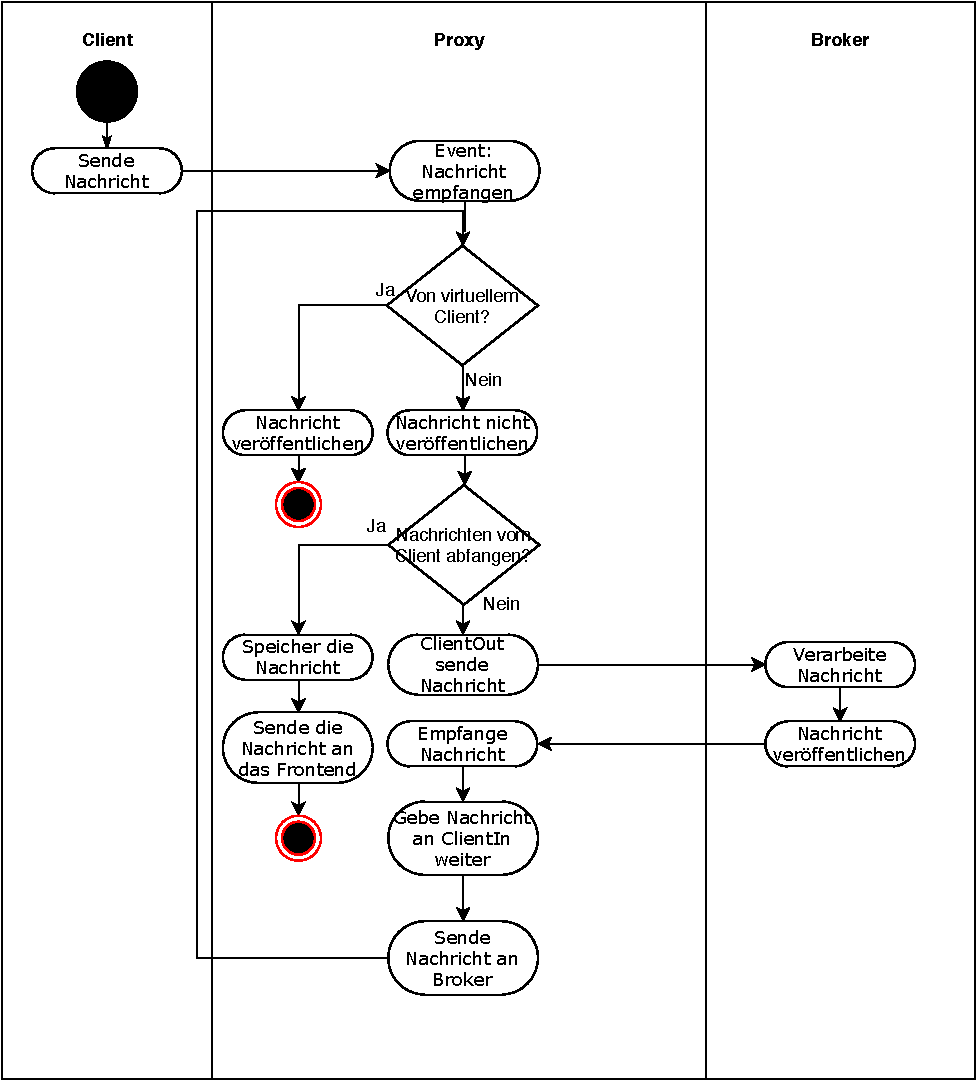
\includegraphics[width=14cm]{tex/bilder/4_konzept/Activity_Message.pdf}
        \captionof{figure}{Aktivitätsdiagramm für das Event \glqq Nachricht erhalten\grqq{}}
        \label{fig:aktivitaetsdiagramm_message}
    \end{figure}
    
    Das Sequenzdiagramm (\ref{fig:sequenzdiagramm}) gibt einen detaillierten Überblick über die Kommunikation der verschiedenen Objekte und deren Interaktionen miteinander.
    Zu beachten ist, dass der Broker auf der linken Seite sowie beide virtuelle Clients Komponenten der zu entwickelnden Software (des Proxys) sind.
    Der Client sowie der Broker auf der rechten Seite repräsentieren externe Geräte, welche sich unter Umständen nicht in dem gleichen Netzwerk befinden und unabhängig vom Proxy arbeiten.
    
    \begin{figure}[!h]%h=direkt danach t=top b=bottom
        \centering
        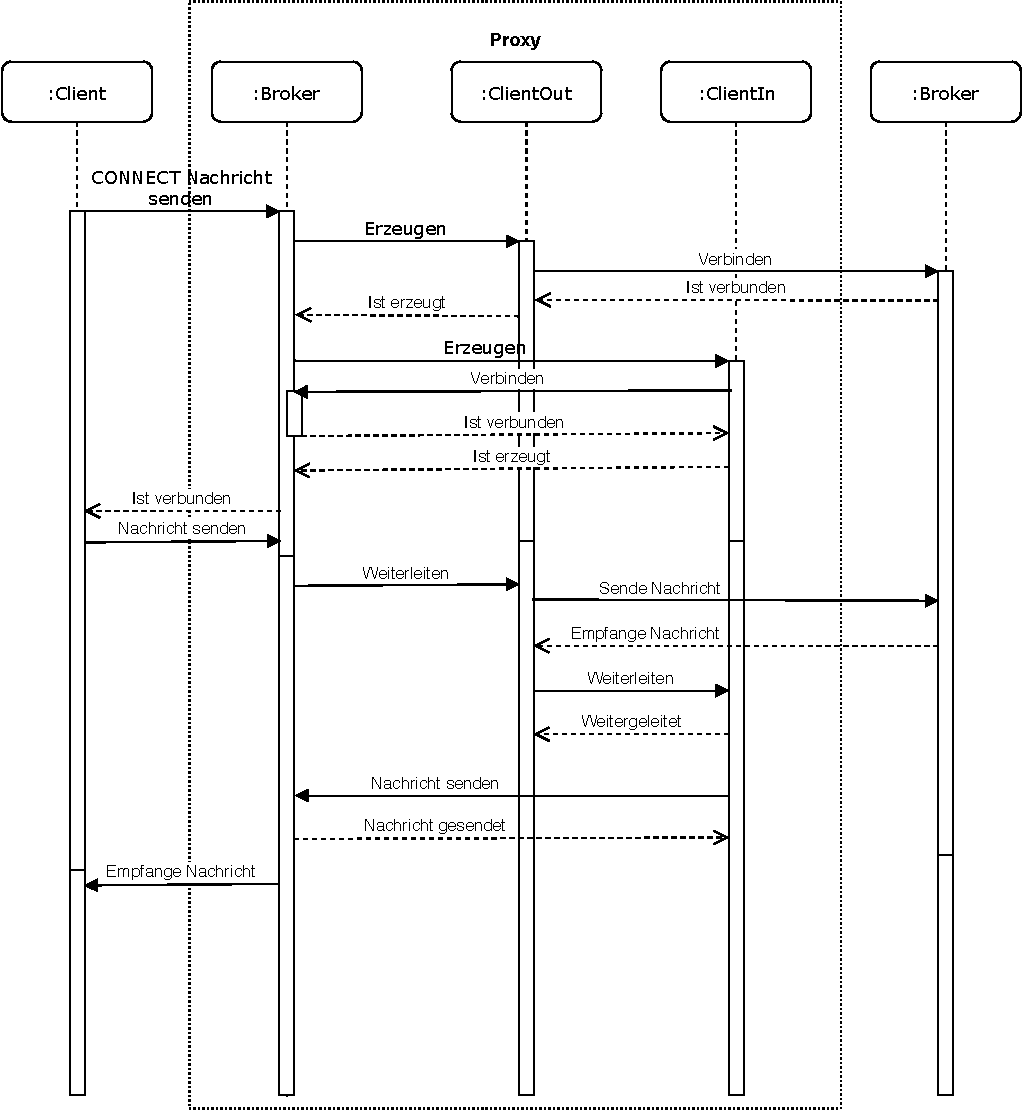
\includegraphics[width=14cm]{tex/bilder/4_konzept/Sequenz.pdf}
        \captionof{figure}{Sequenzdiagramm}
        \label{fig:sequenzdiagramm}
    \end{figure}

\subsubsection{Zusammenfassung}
    Ergebnis des Kapitels ist die Umsetzung der Anforderungen in eine konzeptionelle abstrakte Softwarearchitektur. Hierbei wurden die statische und Laufzeitsicht dargestellt, was als Blaupause für künftige Implementierungen dienen kann. Das Konzept lässt sich in Punkten Programmiersprache, Plattform und Protokoll große Freiheiten. Im Gegensatz dazu legt es klare Vorgaben für die Implementierungen des Proxys fest.
\chapter{Implementierung des Prototypen}

Um das im vorigen Kapitel dargestellte Konzept zu realisieren, lassen sich folgende Hauptaufgaben ausmachen. Im Folgenden wird auf Informationen oder Probleme innerhalb der einzelnen Schritte eingegangen und diese erläutern.

Es wurden viele Open Source Bibliotheken verwendet um den Fokus der Arbeit auf die Neuentwicklung und Lösung der Fragestellung zu legen.

Github wurde im Verlauf der Arbeit verwendet da das Unternehmen wie Chacon et al. in dem Buch Pro Git \cite{Chacon2014} beschreiben, der größte Dienstleister für die Bereitstellung von Git Repositories ist. Neben der Speicherung von Quellcode ist Github ebenfalls eine zentrale Plattform für den Austausch und die Zusammenarbeit von Millionen von Entwicklern. Nicht nur open-source sondern auch closed-source Projekte werden dort gespeichert und mithilfe von Problemverfolgung und Codereviews weiterentwickelt. Für die Verwaltung der Informationen verwendet Github das Versionsverwaltungstool Git und baut somit seine Funktionalität um diese Technologie herum.

\section{Einschränkungen}
Die Software kann nur funktionieren, wenn garantiert werden kann, dass keine effektiven Sicherheitsmaßnahmen verwendet werden. Folgende Maßnahmen würden das mitlesen der Kommunikation verhindern.
\begin{enumerate}
    \item Nur ohne \ac{HPKP}
    
    Auf dem Server wird ein für den Client ausgestelltes Zertifikat hinterlegt. Der öffentlichen Schlüssel oder der \glqq subjectPublicKeyInfo\grqq{}, ein weiterer Schlüssel mit Zusatzinformationen über die Verschlüsselung, dieses Zertifikats wird auf dem Client abgespeichert. Anschließend wird dieser gespeicherte Schlüssel mit jeder Anfrage an den Server mitgeschickt. Anschließend kann der Server die eingehenden Nachrichten mithilfe der Informationen aus dem Zertifikat verifizieren und sicherstellen das sie vom tatsächlichen Ziel kommt \cite{evans_palmer_sleevi_2015}.
    \item Nur wenn der Zertifizierungspfad des SSL Zertifikat (auch \emph{trust chain} genannt) nicht geprüft wird.
    
    Bei Verwendung von TLS ist es möglich, den Client prüfen zu lassen, ob der Server das entsprechende Hersteller Zertifikat besitzt. Jedes gültige Zertifikat muss von einer \ac{CA} ausgestellt werden, welche das Vertrauen und eventuell die Identität des Besitzers verifiziert. Jedoch gibt es auch Implementierungen die vom Zertifikat nur die formalen Details und nicht die Herkunft (also das \ac{CA}) prüfen.
    Dies ermöglicht, dass die Kommunikation trotz eines manuell (also unverifizierbaren) Zertifikats mit den gleichen Details hergestellt werden kann.
\end{enumerate}


%%%%%%%%%%%%%%%%%%%%%%%%%%%%
%Test Client/Broker implementieren
%%%%%%%%%%%%%%%%%%%%%%%%%%%%
\section{Aufsetzen des externen Client und Broker}
    Da zum Zeitpunkt der Entwicklung keine Geräte zur Verfügung standen, wurden ein virtueller Client und Broker erzeugt, die für die Verifizierung im Labor verwendet wurden.
    Auf diese wird im Folgenden Abschnitt eingegangen.

    %Gewählte Sprache für Client und Broker
    Für die Implementierung des virtuellen Clients und externen Brokers bot sich aus folgenden Gründen Python an:
    \begin{itemize}
        \item Die Programmiersprache sollte schnell und mit geringem Aufwand zu verwenden sein.
        \item Sollte bereits über eine \ac{MQTT} Bibliothek verfügen um das Protokoll nicht selbst interpretieren zu müssen.
        \item Der Client sollte anpassbar sein.
        \item Die Sprache sollte auf Linux laufen um ein Ressourcen sparende Verwendung zu ermöglichen.
        \item Sie sollte ebenfalls auf verschiedenen Betriebssystemen lauffähig \emph{cross platform} sein, um auf beliebigen Systemen verwendbar zu sein.
    \end{itemize}
    %https://pdfs.semanticscholar.org/409d/3f740518eafcfaadb054d9239009f3f34600.pdf
    Nach Sanner ist Python ist eine interaktive und objektorientierte Programmiersprache. Sie wird anders als übliche Programmiersprachen somit nicht zuvor kompiliert\footnote{In maschinenlesbare Instruktionen umwandeln.} sondern zur Laufzeit interpretiert.
    Es stehen verschiedene Datenstrukturen aus high-level Programmiersprachen zur Verfügung wie z.B.: dynamische Bindungen, automatisches Memory Management, Klassen, Ausnahmebehandlung. Weiter ist sie eine einfache, leistungsstarke und universelle Programmiersprache, die einen elegante Syntax vorweist. \cite{sanner1999python}
        
    %Open-Source Bibliotheken Client/Broker
    Eclipse Paho ist eine quelloffene Implementierung eines Clients nach dem \ac{MQTT}-Standard. Dieser Client ist in verschiedenen Programmiersprachen verfügbar und bringt abhängig von dieser, ausgewählte Funktionalitäten mit.
    Das Protokol \ac{MQTT} in der Version 5 wird aktuell bereits in der Sprache C, jedoch von keiner anderen Implementierung unterstützt. Python unterstützt Version 3 des Standards und alle weiteren Features abgesehen von \glqq Message persistance\grqq{} und \glqq high availability\grqq{} was jedoch zu Testzwecken nicht benötigt wird. \cite{eclipse_foundation2017}
    Diese Bibliothek vereinfacht das Programmieren der Clients ungemein mithilfe der vordefinierten Klassen und Funktionen.
    Aus diesem Grund kann sehr viel Konfiguriert und somit auf den eigenen Bedarf eingestellt werden. 

    HBMQTT ist ebenfalls eine Implementierung des \ac{MQTT} Standards, allerdings stellt diese Bibliothek auch einen Broker zur Verfügung. Der Vor- und gleichzeitiger Nachteil ist, dass in dieses Framework sehr restriktiv und eingeschränkt Konfigurierbar ist. Dadurch ist es einfach ein Broker aufzusetzen, jedoch nicht ohne weiteres anzupassen.
    \cite{jouanin_2018}
    
%%%%%%%%%%%%%%%%%%%%%%%%%%%%
%Implementieren des Proxys (Backend)
%%%%%%%%%%%%%%%%%%%%%%%%%%%%
\section{Implementierung des Backends}

    Es wurden verschiedene Programmiersprachen für den Proxy verwendet. Diese wurde entsprechend der Anforderungen und dem Einsatzgebiet abhängig gewählt.
    Die wichtigste Unterscheidung liegt an der Trennung von Backend (Server und Logik Komponenten) und Frontend (Webseite oder User Interface).
    Zuerst wird auf die Sprache für das Backend eingegangen.
    
%%%%%%%%%%%
%Visual Studio
%%%%%%%%%%%
    Als Entwicklungsumgebung für das Backend wurde Visual Studio 2017 \cite{microsoft_2019} von Microsoft verwendet. Dadurch sind auch die Projektdateien, die in dem Repository \glqq MQTT-Proxy\grqq{} \cite{eisenschmidt_2019} gefunden werden können, in einem Visual Studio Projektfile (Datei mit einer .sln Endung) definiert.
    
%%%%%%%%%%%
%Anforderungen an die Programmiersprache
%%%%%%%%%%%
    \begin{itemize}
        \item Die Sprache muss verschiedene Bibliotheken mitbringen die Funktionalitäten wie REST-Interface und \ac{MQTT}-Protokoll bereitstellen. Dies ist aufgrund der kurzen Zeit die für diese Arbeit veranschlagt wurde notwendig um alle Features implementiert zu bekommen.
        \item Das Programm muss auf mindestens zwei Plattformen verwendbar sein um den praktischen Nutzen zu steigern.
        \item Es soll eine bekannte Sprache sein, um eine Weiterentwicklung von Dritten zu ermöglichen.
        \item Die Programmiersprache muss dem Autor bereits bekannt sein, um die Einarbeitungszeit minimal zu halten und auch eine entsprechende Qualität zur Verfügung stellen zu können.
    \end{itemize}
%%%%%%%%%%%
%Sprache
%%%%%%%%%%%
    %Welche Sprachen wären basierend darauf möglich/naheliegend gewesen
    Basieren auf diesen Anforderungen stehen Java, C\# und JavaScript zur Auswahl.
    Der Autor hat sich anschließend aus folgenden Gründen für C\# entschieden.
    %Warum sind die Entwickelt worden? / Vorteile Background
    %Was macht die Programmiersprachen aus? / Schwerpunkt
    \begin{itemize}
        \item Die \ac{IDE} Visual Studio und das .NET Framework sind stark in Windows integriert, wodurch die Verwendung dieser unter Windows erleichtert wird.
        \item Das .NET Framework besitzt ein Assembly System bei dem Bibliotheken in einzelne Dateien ausgelagert und dynamisch geladen werden können.
        \item Es ist kein Linking nötigt, da externe Abhängigkeiten zur Laufzeit aufgelöst werden.
        \item Das Paketmanagement System Nuget ermöglicht eine schnelle und einfache Verwaltung sowie Einbindung externer Bibliotheken.
    \end{itemize}
    
    
%%%%%%%%%%%
%Nuget %https://link.springer.com/book/10.1007%2F978-1-4302-4192-8
%%%%%%%%%%%
    NuGet wurde aus den folgenden Vorteilen ausgewählt, welche ebenfalls von Balliauw et al. beschrieben werden \cite{balliauw2012pro}.
    Der sogenannte Paket-Manager unterstützt bei der Verwaltung von Abhängigkeiten, wie zum Beispiel Bibliotheken, mit dem Auflösen von Abhängigkeiten und Versionsproblemen. Versionsprobleme treten dann auf, wenn Bibliotheken Abhängigkeiten mit einer Version < X und eine weitere Bibliothek Version > X benötigen. Ein weitere oft auftretender Fall ist, dass beim Aktualisieren einer Bibliothek die benötigte Version für die Abhängigkeiten erhöht aber nicht ebenfalls aktualisiert wird. Die Folge ist eine defekte Abhängigkeit für die Bibliothek und also ein nicht kompilierbarer Zustand  und somit nicht ausführbares Programm. Zusätzlich übernimmt es auch die Installation durch Suchen, Installieren und Aktualisieren oder Entfernen von gewünschten Paketen. Ein weiterer Vorteil ist, dass der Quellcode öffentlich verfügbar ist und das Tool somit weiter angepasst oder verändert werden kann.
    
%%%%%%%%%%%
%Bibliothek
%%%%%%%%%%%
    NewsoftJSON \cite{newton_king_2013} ist ein quelloffenes Framework für die Serialisierung und Deserialisierung von .NET Framework Objekten.
    Heinzl beschreibt Serialisierung mit folgenden Worten \glqq Unter Serialisierung versteht man die Zerlegung des Status eines Objekts in ein Bytearray.\grqq{} \cite{Heinzl2005}. Allerdings ist es auch möglich dieses Bytearray als strukturierten Text anzeigen zu lassen.
    Dies ermöglicht, ein Nachrichtenobjekt an das Frontend zu übertragen und es dort anschließend wieder darstellen zu lassen.
    
    MQTTNet ist eine quelloffene Implementierung des \ac{MQTT}-Standards in C\# unter der MIT Lizenz\footnote{
    Github beschreibt die Lizenz als einfache freigebige Lizenz mit nur wenigen Einschränkungen wie dem Erhalt von Urheberrechts- und Lizenzhinweisen. Änderungen und größere Werke können unter anderen Lizenzbedingungen und ohne Quellcode verbreitet werden. \cite{github_inc_2019}}.
    Da die Bibliothek MQTTnet \cite{chkr1011_2018},
    welche in dieser Arbeit verwendet wird, die Bridge Funktionalität nicht besitzt ist es notwendig sie selbst zu implementieren. Um das gleiche Ergebnis wie die der Bridge zu erreichen muss an den Broker eine Client Komponente angeschlossen werden der die Kommunikation nach außen steuert und die Antworten weiter verarbeitet. 
    
    WebSocketSharp ist eine C\# Implementierung des WebSocket Protokolls und unterstützt sowohl den Client als auch die Bereitstellung des Server.
    
    Grapevine ist eine .NET Bibliothek die zwei Probleme verfolgt.
    \begin{itemize}
        \item Das einfache einbinden eines REST und HTTP Servers.
        \item Die einfache Verwendung von REST Ressourcen.
    \end{itemize}
    Der Fokus liegt dabei auf der Bereitstellung von Ressourcen über HTTP oder REST für Programme, die einen anderen Schwerpunkt haben und dies nur als Zusatzfunktion benötigen.
    
%%%%%%%%%%%%%%%%%%%%%%%%%%%%
%Implementieren des Proxys (Frontend)
%%%%%%%%%%%%%%%%%%%%%%%%%%%%
\section{Implementierung des Frontends}
    
    Nun wird auf die Programmiersprache für das Frontend, also die Oberfläche eingegangen.
    
%%%%%%%%%%%
%Visual Studio Code
%%%%%%%%%%%
    %https://proquestcombo.safaribooksonline.com/9781484242247
    Zum Entwickeln des Frontends, also der Weboberfläche mit der Nutzer interagieren und die Applikation steuern können, wurde Visual Studio Code \cite{microsoft_2016} verwendet.
    
%%%%%%%%%%%
%Anforderungen an die Programmiersprache
%%%%%%%%%%%
    \begin{itemize}
        \item Es muss möglich sein, einzelne Inhalte auf der Webseite dynamisch, also ohne Aktualisierung der Webseite, austauschen zu können.
        \item Wenn neu abgefangenen Nachrichten im Proxy verfügbar sind, sollen sie automatisch an das Frontend weitergegeben werden und das Datenmodel der Oberfläche automatisch aktualisieren.
        \item Die Oberfläche soll aus Komponenten bestehen und mithilfe dieser einen modularen und strukturierten Aufbau ermöglichen.
        \item Funktionalitäten und Ausprägungen von Komponenten sollen gekapselt sein.
    \end{itemize}
    
%%%%%%%%%%%
%Welche Sprachen wären basierend darauf möglich/naheliegend gewesen
%%%%%%%%%%%
    Durch die existierenden Anforderungen hat sich JavaScript als passend herausgestellt. Dadurch, dass verschiedene Frameworks und Erweiterungen auf Basis von JavaScript existieren, werden im Folgenden noch die konkreten Frameworks auf die Anforderungen untersucht.
    
%%%%%%%%%%%
%Warum Vue.js
%%%%%%%%%%%
    Vue.js \cite{you2018vue} wurde ursprünglich für schnelles Prototyping von Webseiten entwickelt, hat sich aber mit der Zeit in die Liste der beliebtesten Webtechnologien eingereiht. Neben Angular und React, stellt es eine Alternative zum schnellen und leichtgewichtigen Entwickeln mit \ac{MVVM}-Architekturmuster dar. Dies ermöglicht die Wiederverwendung von Code durch Nutzung von Komponenten. Durch die bidirektionale Databindung ist es möglich Änderungen im Clientmodel direkt, ohne Aktualisierung, anzeigen zu lassen. In der gegengesetzten Richtung, werden die Informationen, welche zum Beispiel in Inputfeldern bearbeitet werden können, direkt im Clientmodel abgespeichert. Ein weiterer Vorteil ist die direkte Abbildung vom Datenmodel also Datenstruktur zum ViewModel. Dies ermöglicht auch eine Trennung von UI-Designern und Entwicklern da getrennt entwickelt werden kann ohne Informationen in Bereichen der anderen abändern zu müssen.
    %%%%%%%%%%%%%%%%%%%%%%%%%%%%%%%%%%%%%%%
    % Danke an Moritz für die Infos \.A./ %
    %%%%%%%%%%%%%%%%%%%%%%%%%%%%%%%%%%%%%%%
    
%%%%%%%%%%%
%Bibliothek
%%%%%%%%%%%
    Als Bibliothek wurde Bootstrap-Vue gewählt, um schnell anpassbare Oberflächen erstelle zu können.
    Laut Morehouse \cite{morehouse_2019} ist sie die umfassendste Implementierung von Bootstrap in der Version 4 für Vue.js.
    Bootstrap ist ein quelloffenes Framework, welches fertige Vorlagen und Komponenten für die Erstellung von Webseiten bereitstellt. Der Unterschied zwischen Bootstrap und Bootstrap-Vue besteht darin, dass die vorhandenen Elemente nun als Komponenten in Vue vorhanden sind und somit nicht der ursprüngliche \ac{HTML}-Code\footnote{\ac{HTML} ist die Auszeichnungssprache für das \ac{WWW} \cite{w3c_2017}. Was bedeutet, dass es die grundlegende Sprache für das Erstellen von Webseiten ist.} geschrieben werden muss. Diese Informationen werden automatisch mithilfe der Vue Komponenten generiert.
        
%%%%%%%%%%%%%%%%%%%%%%%%%%%%
%Kommunikation mit Firewall
%%%%%%%%%%%%%%%%%%%%%%%%%%%%
\section{Umsetzung des MITM Proxies}
    %MITM (APR Spoof, DNS, ICMP, FW)
    Es gibt verschiedene Techniken und Möglichkeiten, die Kommunikation so zu verändern, dass ein drittes Gerät die übertragenen Nachrichten mitlesen kann. Ein solches Konzept ist auch unter dem Namen \emph{Man in the Middle} bekannt.
    
    Eine der Möglichkeiten wird auch in dieser Arbeit umgesetzt das die Verbindung vom Client direkt zum Broker aufgebaut wird.
    Mithilfe von Portweiterleitungung in der Firewall \emph{OPNSense} wurden Netzwerkpakete des \ac{IoT}-Gerätes an den Proxy umgeleitet. Hierzu wurde eine Regel erzeugt (siehe \ref{fig:firewall_rule}, die das \emph{source} Attribut jedes eintreffenden Pakets mit der IP-Addresse des Geräts und dem Standard-Port 1883 vergleicht. Bei Übereinstimmung wurde das \emph{destination} Attribut der Pakete umgeschrieben um die Pakete anschließend an den Proxy weiterzuleiten.
    \begin{figure}[h]%h=direkt danach t=top b=bottom
        \centering
        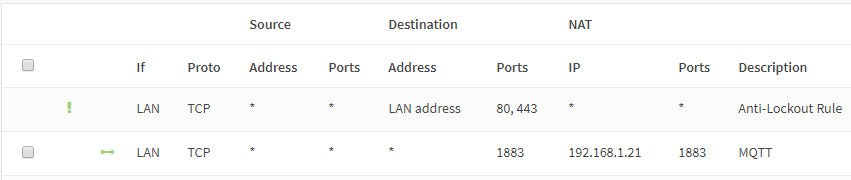
\includegraphics[width=14cm]{tex/bilder/5_implementierung/firewall.PNG}
        \captionof{figure}{Firewallregel zum Umleiten der MQTT-Pakete}
        \label{fig:firewall_rule}
    \end{figure}
\chapter{Validierung}
%Überprüfen der Thesen
%    Szenarien mit erwarteten Ergebnissen vergleichen
%    Ergebnisse über Prototyp bestätigen
    
Um bewerten zu können, ob das entwickelte Programm den in Kapitel 4 genannten Anforderungen entspricht, wird in diesem Kapitel zur Validierung ein virtualisiertes Labor aufgebaut, das einen virtuellen \ac{IoT}-Client, einen virtuellen Broker und den Proxy bereitstellt.

%Szenario, was mit dem Labor versucht wird zu erreichen.
Das Labor bildet die Kommunikation zwischen einem Sensor, welcher sich in der Glühbirne im Wohnzimmer des Nutzer befindet, und dem Broker des Herstellers ab. Der Sensor, im weiteren \emph{Client} genannt, stellt dem Broker jede Sekunde den aktuelle Status zur Verfügung. Der Broker hingegen erwartet den Status eines Clients und veröffentlicht diesen für andere externe Clients.

\begin{figure}[h]%h=direkt danach t=top b=bottom
    \centering
    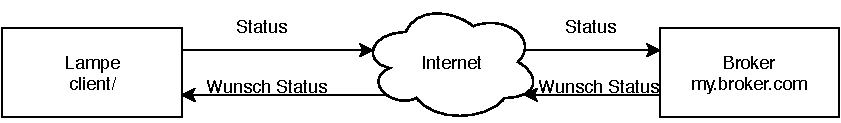
\includegraphics[width=14cm]{tex/bilder/6_validierung/Szenario.pdf}
    \captionof{figure}{Darstellung des Szenarios}
    \label{fig:darstellung-szenario}
\end{figure}

\section{Laboraufbau} \label{Laboraufbau}
    %Warum Virtualisierung/ Virtualisierte Umgebung
    Das Labor wird mithilfe der Virtualisierungslösung \emph{ESXi} %\cite{https://www.vmware.com/de/products/esxi-and-esx.html}
    der Firma \emph{VMware} umgesetzt. Dadurch, dass alle Systeme und Applikationen in sogenannten virtuellen Maschinen laufen, sind sie, obwohl sie auf dem gleichen physikalischen Gerät (Server) laufen können, voneinander unabhängig. Das bedeutet, dass ganze Systeme abgeschottet und auf virtuellen Festplatten (sog. \emph{\acp{VMDK}}) gespeichert und somit auch sehr einfach gesichert oder untereinander ausgetauscht werden können. Durch die dynamische Verteilung von zum Beispiel \ac{CPU} oder RAM ist ebenfalls eine effektivere Nutzung von Hardwareressourcen möglich. Damit wird nur ein Server oder leistungsfähiger Computer benötigt um ganze Systemlandschaften und Netzwerke abzubilden. Des Weiteren ermöglicht es auch, die hier durchgeführten Tests und somit Ergebnisse in der gleichen Umgebung durch die Bereitstellung der Dateien nachvollziehen zu können, ohne selbst Arbeit und Zeit in den Aufbau derselben Systeme investieren zu müssen.
    %Warum mit ESXI
    \emph{ESXi} wurde als Lösung gewählt, da bereits Wissen und Erfahrung im Umgang mit der Lösung vorhanden war. Zusätzlich stand ein Server mit benötigter Leistung bereits zur Verfügung wodurch das Aufsetzen und Konfigurieren eines solchen oder ähnlichen Produkts nicht mehr nötig war.
    
    Die folgenden Voraussetzungen sind notwendig um das Programm ausführen zu können:
    \begin{itemize}
        \item Betriebssystem: ab Windows 7, Linux mit Mono
        \item Abhängigkeiten: .NET Framework v4.6.1, Mono ab 4.2.0.X
        \item Speicher: 50 \ac{MB} frei
        \item RAM: 100 \ac{MB} frei
        \item Prozessor: 2 virtuelle Kerne  mit 2,0 Ghz
        \item Netzwerkkarte: Ja
    \end{itemize}
    
    \subsection{Virtualisierung der Geräte}
    Die in diesem Szenario enthaltenen Systeme sind die Folgenden:
    \begin{table}[h]
        \centering
        \begin{tabular}{c|c|c|c}
            Name & Client & Broker & Proxy \\ \hline
            OS & Debian 9 & Debian 9 & Microsoft Windows 10 \\
            CPU & 1 vCPUs & 1 vCPUs & 4 vCPUs \\
            RAM & 512 \ac{MB} & 512 \ac{MB} & 8 GB \\
            HDD & 5 GB & 5 GB & 50 GB \\
        \end{tabular}
        \caption{Ressourcen der Virtuelle Maschinen}
        \label{tab:ressourcenverteilung}
    \end{table}
    
    Der Client verwendet folgende Software:
    \begin{itemize}
        \item Python 2.7.X
        \item pip-Paket: paho-mqtt
    \end{itemize}
            
    Der Broker arbeitet mithilfe folgender Software:
    \begin{itemize}
        \item Python 3.X, Python3-pip
        \item pip-Paket: hbmqtt
    \end{itemize}
            
    Das Proxy-System, welches die Kommunikation überwacht, benötigt zum Ausführen der Proxy-Anwendung folgende Software:
    \begin{itemize}
        \item Microsoft Visual C++ 2008
        \item Microsoft Visual C++ 2017
        \item .NET Framework 4.6.1
    \end{itemize}
    
    \subsection{Netzwerk}
    Es werden Netzwerke verwendet in denen sich alle Geräte befinden. 
    Das erste Netzwerk beinhaltet den Audit PC, die Proxy Anwendung und den virtuellen Broker sowie die Firewall als Schnittstelle zum zweiten Netzwerk.
    Die Firewall spannt ein \ac{VLAN} auf, in dem sich der Client befindet. Mittels Portweiterleitung\footnote{Pakete, die an einen spezifizierten Port beinhalten, werden an ein festgelegte Adresse weitergeleitet.} leitet es den Datenverkehr des Clients zum Proxy um. %TODO FRAGEN OB QUELLE NOTWENDIG
    
    \begin{figure}[h]%h=direkt danach t=top b=bottom
        \centering
        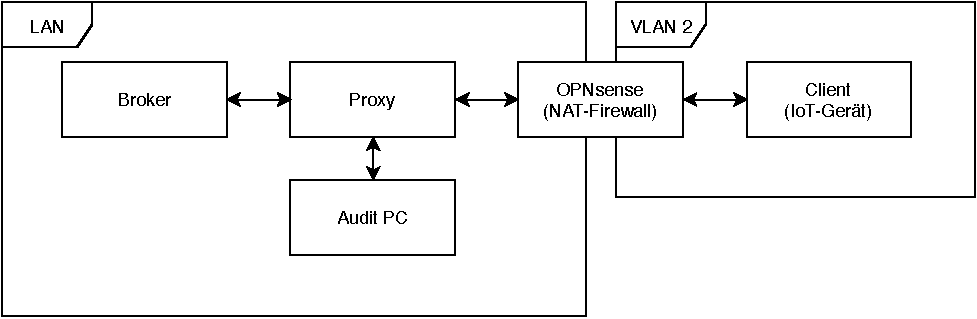
\includegraphics[width=14cm]{tex/bilder/6_validierung/Netzwerkdiagramm.pdf}
        \captionof{figure}{Darstellung des virtuellen Netzwerks}
        \label{fig:virtuelles_netzwerk}
    \end{figure}
    
    \subsection{Konfiguration der Software} \label{KonfigurationDerSoftware}
    %Konfiguration
    Das Projekt ist im Standard auf Prozessoren mit x86-Befehlssatz ausgerichtet, kann allerdings bei Bedarf auch auf Prozessoren mit x64-Befehlssatz durch Änderung der entsprechenden Einstellung in Visual Studio geändert werden.
    Eine Unterstützung für weitere Architekturen ist durch die Installation plattformübergreifender Implementierungen von Mono und Python möglich. Auch muss hierzu in Visual Studio die Zielarchitektur auf "Any CPU" gesetzt werden. 
    Zusätzlich ist zur Ausführung der Anwendung ein privilegierter Account erforderlich, um die Berichtigung für Zugriff auf die erforderlichen Ports zu erhalten.
    
    Es werden Port 1883 für die Kommunikation über das \ac{MQTT}-Protokoll und Port 80 für die \ac{REST} Schnittstelle und einen Webserver, der die Weboberfläche bereitstellt, benötigt.
    Der Proxy ist ausschließlich über die Adresse \glqq 127.0.0.1\grqq{} oder \glqq localhost\grqq{} erreichbar, da keine Benutzerauthentifizierung implementiert wurde. Im lokalen Netz oder bei Bereitstellung über eine öffentlich erreichbare Adresse, kann eine unberechtigte Verwendung nicht ausgeschlossen werden. Daher wird dies auch nicht empfohlen. Sofern jedoch die Notwendigkeit bestehen sollte, ist es möglich die Adresse im Quellcode durch die lokale IP-Adresse des Gerätes, auf dem der Proxy ausgeführt wird, auszutauschen, um eine parallele oder externe Verwendung zu ermöglichen.

    Für den Broker wird eine Konfigurationsdatei, wie in Listing \ref{fig:broker_config} zu sehen, angelegt. Diese definiert unter Anderem, wie viele Verbindungen akzeptiert werden und auf welchem Interface gelauscht wird. Anschließend wird noch die Authentifizierung deaktiviert und mithilfe von einem Plugin werden \emph{Topics} von eingehenden Nachrichten automatisch erzeugt. 
    \begin{figure}[h]
        \begin{lstlisting}
            listeners:
              default:
                max-connections: 5000
                bind: 0.0.0.0:1883
                type: tcp
            auth:
              allow-anonymous: true
            topic-check:
              enabled: True
            plugins:
              - topic_taboo
        \end{lstlisting}
        \captionof{lstlisting}{Broker Konfiguration}
        \label{fig:broker_config}
    \end{figure}

\section{Ausführung und Bewertung}
Auf Abbildung \ref{fig:client_messages} ist der erstellte virtuelle Client zu sehen, welcher Nachrichten über den Proxy an den Broker schickt.
%Was für Nachrichten
Nach dem erfolgreichen Abonnieren des \emph{Topics}, sendet der virtuelle Client jede Sekunde eine Nachrichten mit dem aktuellen Status an den Broker. Kurz darauf veröffentlicht der Broker diese Nachricht in dem abonnierten \emph{Topic}. Aus diesem Grund erhält der Client anschließend dieselbe Nachricht wieder zurück. Abhängig vom Szenario muss der Client nicht an seinen Veröffentlichungen interessiert sein und kann auch andere \emph{Topics} \emph{"subscriben"} (abonnieren).
\begin{figure}[!h]%h=direkt danach t=top b=bottom
    \centering
    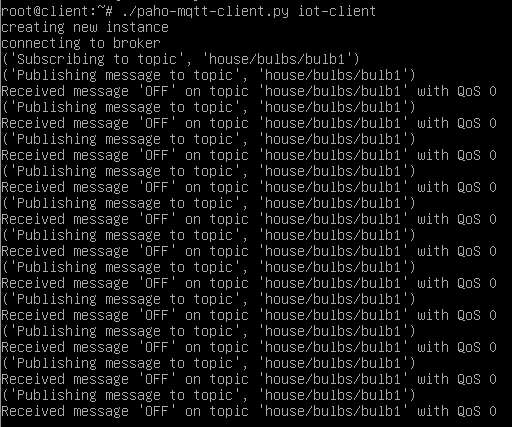
\includegraphics[width=10cm]{tex/bilder/6_validierung/ClientMessages.png}
    \captionof{figure}{Darstellung des gesendeten Nachrichten vom Client}
    \label{fig:client_messages}
\end{figure}

In Abbildung \ref{fig:broker_connections} ist die Initialisierung des Brokers zu sehen. Er wird mithilfe einer Konfigurationsdatei gestartet (siehe \ref{KonfigurationDerSoftware}). Anschließend wird angezeigt, dass erst eine und danach eine zweite Verbindung zum Broker hergestellt wurde. Diese Verbindungen werden allerdings nicht mit dem virtuellen Client, sondern den Clients des Brokers aufgebaut.
\begin{figure}[!h]%h=direkt danach t=top b=bottom
    \centering
    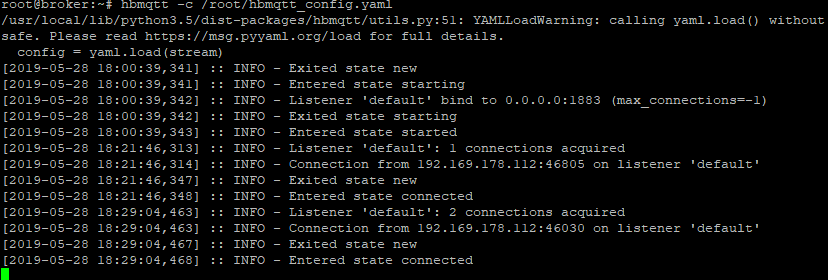
\includegraphics[width=14cm]{tex/bilder/6_validierung/BrokerConnections.png}
    \captionof{figure}{Darstellung der Client-Verbindungen beim Broker}
    \label{fig:broker_connections}
\end{figure}

Der Proxy zeigt, wie Abbildung \ref{fig:proxy_messages} zu entnehmen ist, beim Erhalt einer Nachricht, vom virtuellen Client (\ac{IoT}-Gerät), sowie vom Proxy Client (\emph{ClientIn}), deren Inhalt an.
Darüber hinaus, zeigt er auch weitere Aktionen des \emph{ClientManagers} und der virtuellen Client an.
Mithilfe der Nachrichten lassen sich der Ablauf des Programms und etwaige Fehler nachvollziehen. Diese Ausgabe kostet jedoch vergleichsweise viel Leistung, woraus die in \ref{Laboraufbau} aufgeführten Systemanforderungen resultieren. 
\begin{figure}[!h]%h=direkt danach t=top b=bottom
    \centering
    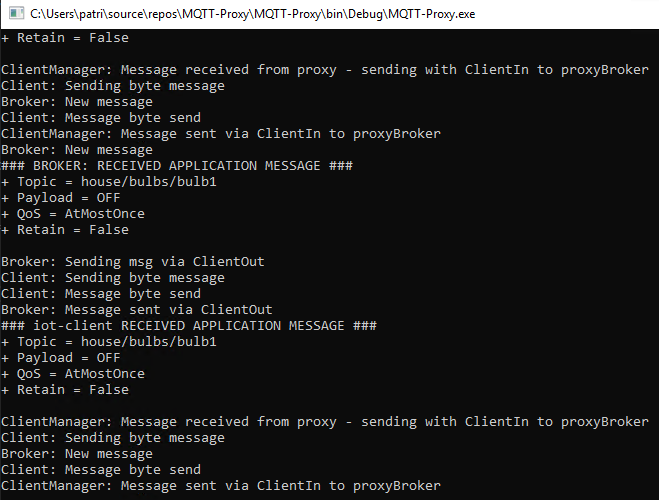
\includegraphics[width=12cm]{tex/bilder/6_validierung/ProxyMessages.png}
    \captionof{figure}{Darstellung der Nachrichten verarbeitet vom Proxy}
    \label{fig:proxy_messages}
\end{figure}

Das Frontend des \emph{Interceptors}, welches auf Abbildung \ref{fig:frontend_messages} zu sehen ist, ist die Kernkomponente der Software. Sie zeigt alle abgefangenen Nachrichten und ermöglicht, diese zu filtern, editieren und erneut zu versenden. Die Nachrichten werden chronologisch untereinander aufgelistet. Pro Nachricht werden dem Nutzer alle wichtigen Inhalte bereitgestellt.
\begin{figure}[!h]%h=direkt danach t=top b=bottom
    \centering
    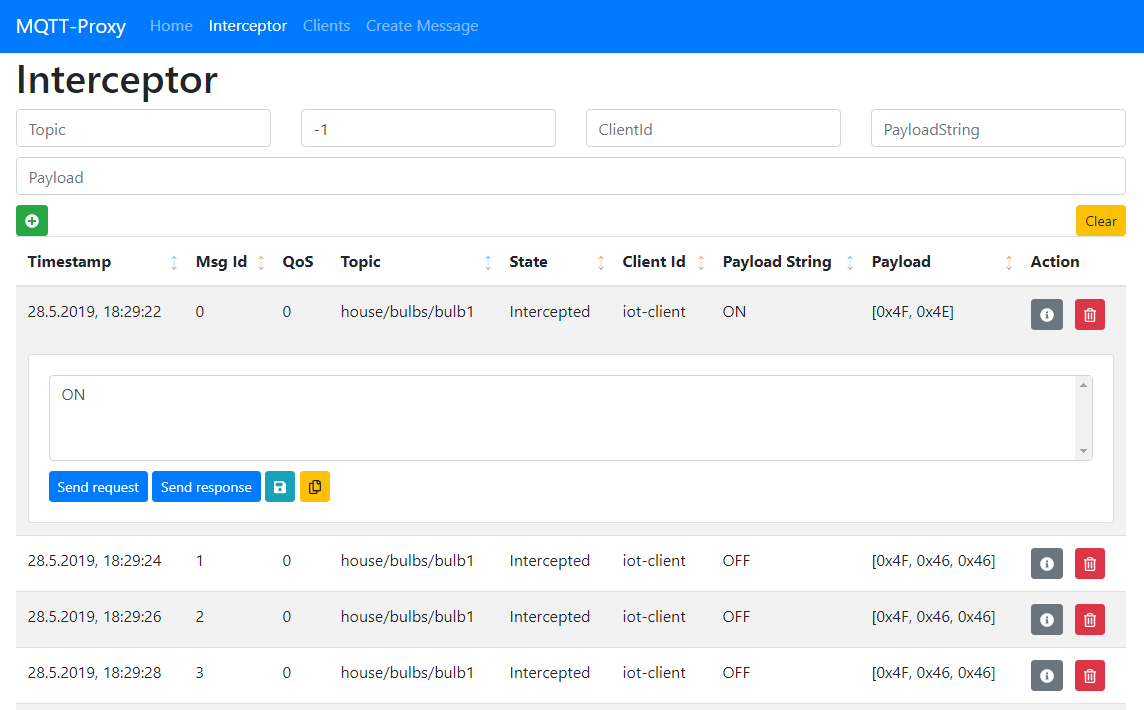
\includegraphics[width=14cm]{tex/bilder/6_validierung/FrontendInterceptor.png}
    \captionof{figure}{Darstellung der Nachrichten im Frontend}
    \label{fig:frontend_messages}
\end{figure}

\section{Performance}
    Hier wird die Performance des Proxys analysiert, um Hinweise auf Skalierbarkeit und zur Ausführung notwendige Ressourcen zu erhalten.
    Folgende Messwerte wurden mithilfe des \emph{Visual Studio Profilers} auf der \ac{VM} des Proxys erfasst.
    
    \begin{enumerate}
        \item Ohne Clients:
        Solange das Programm im Leerlauf arbeitet, also nur Events registriert, die auf Einwirkung anderer Komponenten warten, benötigt es rund 19 \ac{MB} \ac{RAM} und hat eine maximale \ac{CPU} Auslastung von einem Prozent.
        \item Mit einem Client:
        Sobald der erste Client sich verbunden hat, wir nur ein \ac{MB} mehr \ac{RAM} benötigt, in einer Summe von 20 \ac{MB} resultiert. Im Gegensatz dazu werden nun nach der ankommenden Nachricht vom \ac{IoT}-Client alle Funktionen des Programms ausgeführt. Dies führt zu einer Erhöhung beim Ausführen der "Connect"-Funktion auf 20 Prozent und anschießend maximal 17 Prozent.
        \item Mit zwei Clients:
        Kommt nun ein weiterer Client dazu, sodass nun zwei Clients mit dem Proxy verbunden sind, steigt der \ac{RAM}-Verbrauch weiterhin nur um einen Prozent auf 21 \ac{MB} an. Die maximale \ac{CPU} Auslastung steigt jedoch auf 33 Prozent an, was eine Steigerung um 95 Prozent darstellt. Dies ist unter anderem auf ein aktuelles Problem in der Proxy-Implementierung %\cite{https://github.com/Patrick-DE/MQTT-Proxy/issues/3}
        zurückzuführen, das dazu führt, dass jeder Client die Antworten aller Clients an den Proxy schickt. Dies bedeutet, dass Antworten des externen Brokers doppelt erfasst und publiziert werden.
        Bei genauerer Analyse beider am Ansteigen beteiligten Funktionen, ist zu erkennen, dass der größte Ressourcenbedarf bei den folgenden Funktionen zu verorten ist:
        \begin{itemize}
            \item Für 30 Prozent der maximalen \ac{CPU}-Auslastung des Programms ist die "Connect"-Funktion verantwortlich. Die "Connect"-Funktion wird aufgerufen, sobald sich ein \ac{IoT}-Client bei dem Proxy registriert. Sie beinhaltet mehrere kaskadierende Methodenaufrufe, womit der Verbindungsauf von Clients ressourcenintensiv wird.  
            \item Für 57 Prozent der maximalen \ac{CPU}-Auslastung des Programms ist die Systemfunktion \emph{"Console.WriteLine()"} Funktion verantwortlich. Da in diesem Programm viele Informationen an die Konsole zur Information an den Entwickler oder Nutzer weitergereicht werden, ist dies die Hauptursache dafür, dass das Programm die oben genannten \ac{CPU}-Auslastung aufweist. Zu bemerken ist jedoch, dass diese nur den maximalen Wert anzeigen, welcher nur vorhanden ist, wenn Nachrichten an den externen Broker weitergeleitet werden.
        \end{itemize}
    \end{enumerate}
    %TODO Visual Studio Profiler Screenshot von timeline mit marker auf 1 2 3 Clients
\chapter{Ergebnis}
Was sind die gewonnenen Erkenntnisse?
Was kann ich jetzt damit anstellen?
Hab Software erstellt um
Bruteforcen
Fuzzen
Crashen
Schwachstellen finden
Information disclosure
\chapter{Fazit}
%Zusammenfassung
Es wurde ein Konzept für eine Software erstellt, die einen Proxy realisiert und von System-, Netzwerkadministratoren sowie Security Auditoren verwendet werden kann um deren Arbeit zu erleichtern. Dieses Konzept kann nicht nur unabhängig von der Sprache entwickelt, sondern auch auf verschiedenen Plattformen ausgeführt werden. Eine weitere Besonderheit ist, dass selbst das Protokoll dank der Modularität ausgetauscht werden kann und somit weitere Protokolle unterstützt.
Die Software, welche im Rahmen der Arbeit entwickelt wurde, erfüllt die erfassten Anforderungen und unterstützt mithilfe verschiedener Funktionen (wie ...) die Nutzer bei Ihrer Arbeit. Es wurde jedoch eine Schwächen bei der Überwachung identifiziert, da Nachrichten nicht ohne einen aktiven Eingriff in die Kommunikation aufgezeichnet werden können.

%Was gemacht
%Was gelernt
%Wichtigsten Punkte aus dem Ergebnis mit Verweis
%Bewertung der wichtigsten Punkte, gut/ schlecht? wie verbessern

\section{Ausblick}
%Wo kann es in Zukunft genutzt werden?
Die Software kann in Zukunft in Netzwerken eingesetzt werden, um die Kommunikation eines oder mehrerer Geräte zu einem Broker zu überprüfen.
Weiter kann sie eingesetzt werden, um mithilfe verschiedener Methoden (zum Beispiel: Fuzzen, Bruteforce, Replay) den Endpunkt des Gerätes oder des Brokers auf Schwachstellen zu prüfen. Somit kann die Sicherheit der Geräte durch melden der fehlerhaften Funktionen an den Hersteller oder Entwickler erhöht werden. Weiter ist es möglich herauszufinden, welche Daten an den Hersteller übertragen werden um somit mehr Transparenz, in Bezug auf Themen rund um den Datenschutz, zu ermöglichen.

\section{Weiterführende Arbeiten}
%Was wäre noch als Erweiterung möglich
%konkrete Projekte zur Erweiterung/ Verbesserung vorschlagen
Im Laufe der Arbeit wurden verschiedene Ideen und Konzepte über potenzielle Erweiterungen entwickelt, welche im Folgenden aufgeführt werden.
Es könnte ein \emph{Discovery-Modus} hinzugefügt werden, der in unbekannten Netzwerkverbindungen, anhand von speziellen Mustern, die implementierten Protokolle automatisch erkennen kann. Zusätzlich soll die Erkennung auch umschließende Transporttechnologien erkennen können und somit geschachtelte Verbindungen ebenfalls erkennen können. Dies würde in unbekannten oder neuen Netzen das Suchen der Geräte beschleunigen und die Überwachung präziser und vollständiger machen.
Dadurch, dass Anfang 2019 MQTT in der Version 5 verabschiedet wurde, wäre es notwendig in Zukunft eine Unterstützung für das neue Protokoll hinzuzufügen um auch die Kommunikation der neueren Geräte lesen zu können \cite{mqtt_org_2019}.
Darauf aufbauend könnte eine automatisierte Analyse der Protokolle erfolgen und auf Basis der erkannten \ac{MQTT} Version der korrekte Dekoder ausgewählt werden. Dies würde die Nutzereingabe bezüglich der verwendeten Version pro Client überflüssig machen und das Programm komfortabler somit gestalten.

% ------------------------------------------------------------------

\label{lastpage}

% Neue Seite
\cleardoublepage

% Backmatter mit normalem Zeilenabstand setzen
\singlespacing

% Römische Ziffern für die "Back-Matter", fortlaufend mit "Front-Matter"
\pagenumbering{roman}
\setcounter{page}{\value{frontmatterpage}}

% Abkürzungsverzeichnis
\addchap{\hsmaabbreviations}
% Die längste Abkürzung kann in die eckigen Klammern
% bei \begin{acronym} geschrieben, um einen hässlichen
% Umbruch zu verhindern
\begin{acronym}[IEEE]
\acro{IoT}{Internet of Things}
\acro{MITM}{Man in the Middle}
\acro{MQTT}{Message Queuing Telemetry Transport}
\acro{OWASP}{Open Web Application Security Project}
\acro{DNS}{Domain Name System}
\acro{DNSSEC}{Domain Name Service Security Extention}
\acro{VS}{Visual Studio}
\acro{VC}{Visual Studio Code}
\acro{REST}{Representational State Transfer}
\acro{RAM}{Random Access Memory}
\acro{VMDK}{Virtual Machine Disk}
\acro{VM}{Virtuelle Maschine}
\acro{PTES}{Penetration Testing Execution Standard}
\acro{RAT}{Remote Access Tool}
\acro{ZAP}{Zat Attack Proxy}
\end{acronym}


% Tabellenverzeichnis erzeugen
\cleardoublepage
\phantomsection
\addcontentsline{toc}{chapter}{\hsmalistoftables}
\listoftables

% Abbildungsverzeichnis erzeugen
\cleardoublepage
\phantomsection
\addcontentsline{toc}{chapter}{\hsmalistoffigures}
\listoffigures

% Listingverzeichnis erzeugen. Wenn Sie keine Listings haben,
% entfernen Sie einfach diesen Teil.
\cleardoublepage
\phantomsection
\addcontentsline{toc}{chapter}{\hsmalistings}
%\lstlistoflistings

% Literaturverzeichnis erzeugen
\begingroup
\cleardoublepage
\begin{flushleft}
\let\clearpage\relax % Fix für leere Seiten (issue #25)
\printbibliography
\end{flushleft}
\endgroup

% Index ausgeben. Wenn Sie keinen Index haben, entfernen Sie einfach
% diesen Teil.
\cleardoublepage
\phantomsection
\addcontentsline{toc}{chapter}{\hsmaindex}
\printindex

% Anhang. Wenn Sie keinen Anhang haben, entfernen Sie einfach
% diesen Teil.
%\appendix
%\chapter{Erster Anhang}

Hier ein Beispiel für einen Anhang. Der Anhang kann genauso in Kapitel und Unterkapitel unterteilt werden, wie die anderen Teile der Arbeit auch.


\end{document}
